% !TEX TS-program = xelatex
% !TEX encoding = UTF-8
\documentclass[12pt,oneside]{report}
\usepackage[letterpaper, margin=1in]{geometry} % smaller margins
\usepackage[nottoc,chapter]{tocbibind} % adds entries for the list of figs, list of tables, and bib to the TOC
\usepackage[titletoc]{appendix} % adds "Appendix" before the appendix letter in TOC
\usepackage[parfill]{parskip} % begin paragraphs with empty line, not an indent
\usepackage[compact]{titlesec}
%\usepackage{fancyhdr} \pagestyle{fancy} \fancyhf{} %\lhead[]{} \chead[]{} \rhead[]{} \lfoot[]{} \cfoot[]{\fancyplain{}{\osf \thepage}} \rfoot[]{}  %\cmd[oddpage]{evenpage}
\usepackage{natbib, graphicx, color, url, fontspec, ragged2e, setspace, paralist, float, array, longtable, tabu, booktabs, multicol, multirow, titling}  % \setuldepth{x} tabularx, siunitx, 
\usepackage[hidelinks,pdfpagelabels,xetex]{hyperref}
\hypersetup{
    pdftitle={Prosody, familiarity and intelligibility in speech perception},
    pdfauthor={Daniel R. McCloy},
    pdfsubject={Linguistics},
    pdfkeywords={phonetics, speech perception, prosody, intelligibility, familiarity},
    bookmarksnumbered=true,
    bookmarksopen=true,
    bookmarksopenlevel=1,
    colorlinks=false,
    pdfstartview=Fit,
    pdfpagemode=UseOutlines,
    unicode=true,
}
\usepackage{doi}

% setup handling of code
\usepackage[chapter]{minted} 
\usemintedstyle{default}
\renewcommand\listingscaption{Script}
\renewcommand\listoflistingscaption{List of Scripts}
%FROM THE tocbibind DOCUMENTATION (implementation based on listings package, not minted... should look at listings source code to know how to translate this)
%\renewcommand{\lstlistoflistings}{\begingroup
%	\tocfile{\lstlistingname}{lol}
%\endgroup}
%FROM THE DEFINITION OF \listoflistings (in the minted documentation)
%\providecommand\listoflistings{\listof{listing}{\listoflistingscaption}}


% fonts & formatting
\setmainfont[Numbers={Lining}]{Linux Libertine O} \setmonofont{M+ 1m medium} %\setmonofont{Linux Libertine Mono O}
\newenvironment{itm}{% just like itemize, but with bullets flush left with surrounding text
	\setlength{\leftmargini}{0.5em}%
	\setlength{\leftmarginii}{1em}%
	\setlength{\leftmarginiii}{1.5em}%
	\begin{itemize}}{\end{itemize}%
}
\renewcommand{\labelitemi}{•} \renewcommand{\labelitemii}{◦} \renewcommand{\labelitemiii}{—} % redefine default bullets
\renewcommand{\url}{\begingroup \def\UrlLeft{}\def\UrlRight{}\urlstyle{same}\Url}
\newcommand{\term}[1]{“#1”} % first occurrence of technical terms
\newcommand{\lat}[1]{\textit{#1}} % foreign words
\newcommand{\ac}[1]{\textsc{#1}} % acronyms
% \newcommand{\ac}[1]{\MakeUppercase{#1}}

% formatting for section & subsection headings and table captions
\titleformat{\chapter}{\LARGE\bfseries\doublespacing}{Chapter \thechapter.}{0.6em}{}
\titlespacing*{\chapter}{0pt}{-50pt}{*0} % -50pt is a hack to undo the default (which for \chapter won't be undone by just using *0)
\titlespacing*{\section}{0pt}{*0}{*0}
\titlespacing*{\subsection}{0pt}{*0}{*0}
\titlespacing*{\subsubsection}{0pt}{*0}{*0}

% table caption related tweaks
\setlength{\LTcapwidth}{\textwidth} % longtables only
\setlength{\extrarowsep}{0.1em}

% hack the section heading names
\renewcommand{\contentsname}{\bfseries\LARGE{Table of Contents}}
\renewcommand{\abstractname}{
	\normalfont
	\begin{spacing}{1}
	\begin{centering}
	University of Washington\\ \vskip 2em%
	\textbf{Abstract}\\ \vskip 2em%
	\thetitle \\ \vskip 2em%
	\theauthor \vskip 2em%
	Chair of the Supervisory Committee:\\Professor Richard A. Wright\\Department of Linguistics \vskip 2em%
	\end{centering}
	\end{spacing}
}

% % % VARIOUS USEFUL UNICODE POINTS FOR COPY/PASTE % % %
% ×±≠ — – ‣•◦◆◇■◼◾▪□◻◽▫▶▸▷▹¹²³⁴⁵⁶⁷⁸⁹⁰⁺⁻⁼⁽⁾ⁱⁿ₀₁₂₃₄₅₆₇₈₉₊₋₌₍₎ₐₑₒₓₔ ←↑→↓↔↕↚↛⇋⇌⇐⇑⇒⇓⇔⇕⇍⇏⇎⇠⇡⇢⇣⇦⇧⇨⇩⟵⟶⟷⟸⟹⟺  ∀ ∃ ∄ ∅ ∈ ∉ ⟦ ⟧ ⊂ ⊃ ⊆ ⊇ ⟨ ⟩ ⟪ ⟫ ≝ ∿ ≃ ≄ ≈ ≉ ≤ ≥ ≪ ≫ ≺ ≻ ⊀ ⊁ ≼ ≽ 𝒫  ❇ ❈

\title{Prosody, familiarity and intelligibility in speech perception}
\author{Daniel~Robert~McCloy}
\date{2013}
\begin{document}
\RaggedRight
\begin{spacing}{2}

%\frontmatter
\pagenumbering{roman}
% % % % %  TITLE PAGE   % % % % %
\begin{titlepage}
	\begin{center}
	\thetitle \\ \vskip 2em
	\begin{tabular}[t]{c} \theauthor \end{tabular} \\	\vskip 3em
	A dissertation\\ submitted in partial fulfillment of the\\ requirements for the degree of\\ \vskip 2em
	Doctor of Philosophy\\ \vskip 3em
	University of Washington\\
	\thedate \\ \vskip 3em
	Reading Committee:\\ Richard A. Wright, Chair\\ Frederick J. Gallun\\ Sharon L. Hargus\\ Gina-Anne Levow\\ \vskip 3em
	Program Authorized to Offer Degree:\\ Linguistics
	\end{center}%
\end{titlepage}
\thispagestyle{empty}

% % % % %      ABSTRACT     % % % % %
\begin{abstract}
Abstract text goes here.  350 words max.  Double space: abstract, dedication, acknowledgements, table of contents, and body of the manuscript, except for quotations as paragraphs, captions, items in tables, lists, graphs, charts. Single space: footnotes/endnotes, bibliographic entries, lists in appendices.
\end{abstract}

% % % % %  TABLE OF CONTENTS  % % % %
\tableofcontents

% % % % %  LIST OF FIGURES  % % % % %
\listoffigures

% % % % %  LIST OF TABLES   % % % % %
\listoftables

% % % % %  LIST OF LISTINGS % % % % %
\listoflistings % unnecessary since all scripts are in appendices

% % % % %  ACKNOWLEDGMENTS  % % % % %
\chapter*{Acknowledgments}
First and foremost I thank my advisor, mentor, and dissertation chair, Richard Wright.  For the last three years he has (among other things) challenged, inspired, critiqued, funded, encouraged, frustrated, and befriended me.  One of the main reasons I finished graduate school was that I truly enjoyed going to our meetings.  I also owe a large debt to the other members of my dissertation committee: Erick Gallun, Sharon Hargus, and Gina-Anne Levow, who guided me with keen questions along the way, and struggled through my inelegant draft prose to help me refine this work.  I would be remiss if I failed to also mention Pam Souza, who has been a great collaborator, and who showed me by her own example that science is at its best when we practice it in the service of humanity.  Jennifer Haywood and Gus McGrath get special mention here as well for their work on the corpus; Gus in particular for having so quickly transitioned from student to trainee to collaborator, and for doing so much of the dirty work that arises when creating spoken corpora that are fit for public consumption.

My colleagues in the UW Linguistics Department have been fine companions, and I have profited from many stimulating discussions over the years.  Special thanks go to Bill McNeill, Julia Miller, Michael Goodman, Valerie Freeman, Lisa Tittle, Sarala Puthuval, Josh Crowgey, and most especially Darren Tanner and Steve Moran.  Most of my conversations with these folks had little to do with my dissertation research, but rather were a source of enrichment and distraction when it was sorely needed.  To the extent that I seem like a well-rounded scholar, it is often because of the little facets of knowledge that I gleaned from each of them.  

I must also acknowledge my dear friends outside of academia, who for several years have tolerated my absence from parties, dinners, concerts, openings, performances and festivals, and yet still embraced me fondly when I did manage to show up once in a while.  My parents have been especially tolerant in this regard, and deserve thanks for so much more than I can describe here.

Along my winding path through education, I have had a number of gifted teachers who quietly inspired me to remain curious and to someday be as good a teacher as they were.  I have always wanted to acknowledge them publicly; this seems as good a place as any.  Thanks to (in chronological order): Sherry Brown (chemistry, grade 10), David Adams (calculus), Dennis Lamb (Greek and Roman literature), Bill Moody (cellular neurobiology), Larry BonJour (epistemology), Bill Talbott (moral and social philosophy), David Knechteges (Chinese literature), Bi Nyan-Ping (Chinese language), Zev Handel (Chinese historical linguistics), and Chris Stecker (psychoacoustics).

% % % % %     DEDICATION    % % % % %
\chapter*{Dedication}
To Sarala, \textit{sine qua non}.


%\mainmatter
% % % % % % % % % % % % % % % % %
% % % % %  INTRODUCTION   % % % %
% % % % % % % % % % % % % % % % %
\pagenumbering{arabic}
\chapter{Introduction}
\section[Overview]{Overview of the thesis \label{sec:Overview}}
Some introductory text here...

\section[Abbreviations \& acronyms]{Abbreviations and acronyms used in the thesis \label{sec:Abbr}}
Following is a table of acronyms and abbreviations used in this thesis.  I have endeavored to spell out each acronym at the point it is first used in the document, but I cannot be certain that I have succeeded in this task, and in any event there will always be readers who choose to skip certain sections, or whose memory for new terminology is imperfect.  I hope this list is useful to them.

\begin{table}
	\caption[Abbreviations and acronyms]{Abbreviations and acronyms used in the thesis \label{tab:Abbr}}
	\centering
	\begin{tabu} to \textwidth [c]{X[c] X[5]}
		\toprule
		\rowfont[c]{\bfseries} Abbreviation & Explanation\\
		\midrule
		\fo & Fundamental frequency (of speech)\\
		F2×F1 & The acoustic space defined by the center frequencies of the first and second formants of sonorant speech sounds (usually vowels)\\
		\ac{rms} & Root mean square (a method of measuring sound power)\\
		\ac{snr} & Signal-to-noise ratio\\		
		\bottomrule
	\end{tabu}
\end{table}

\chapter{Background}
This chapter presents a brief overview of relevant literature on speech intelligibility, prosody, and talker familiarity.  Because the experiments described in this thesis involved speech obscured by background noise, particular attention is given to the perception of speech-in-noise.  The discussion of talker familiarity touches on both short-term familiarity (i.e., training studies) and long-term familiarity.  Finally, the discussion of prosody addresses pitch, loudness, and duration as they relate to speech perception.

\section{The intelligibility of speech in noise}
Quantitative measurements of auditory masking began in the 1920s with the seminal experiments of \citet{WegelLane1924}, who described the masking of one pure-tone signal by a second pure-tone signal of different frequency.  Studies of speech masking followed with the work of \citet{Miller1947}, \citet{Cherry1953}, Tolhurst \citep{BlackEtAl1953}, Hirsh \citep{HirshEtAl1954}, Stevens \citep{HawkinsStevens1950}, and others.  %TODO: say what they did
Since then, numerous factors have been found to impact the intelligibility of speech in noise.  In this section, those factors are discussed in four broad categories: those related to masker signal type, those related to the talker, those related to the listener, and those related to the target signal content.

\subsection{Noise maskers and speech maskers: energetic and informational masking}
Early masking experiments \citep[e.g.,][]{HawkinsStevens1950,Tolhurst1957,PollackPickett1958} were often performed with noise maskers: random (gaussian) signals, usually without any amplitude modulation (“stationary maskers”) or frequency shaping (“white noise maskers”).  Masking due to any such random signal is typically termed “energetic masking”, reflecting the idea that the masking is a consequence of elevated signal detection thresholds in the auditory filters of the cochlea \citep{DurlachEtAl2003}.  However, most everyday situations involve listening to speech in the presence of competing speech streams — a situation poorly modeled by stationary white noise maskers, since real speech is both amplitude modulated and frequency shaped (indeed, the frequency shaping is itself dynamic).  

When speech is used as a masker, the amplitude modulations in background speech create temporal variations in \snr\ of the signal that can offer “glimpses” of the target stream.  The existence of such glimpses make speech a (potentially) worse masker than stationary noise, since listeners can use such glimpses to reconstruct neighboring spans of the target stream that were less clearly heard (based on lexical knowledge, phonotactics, contextual probabilities, etc., \citealt{XXX}).  Thus it is surprising that background speech is in fact a better masker than background noise, provided a fair comparison is made by amplitude-modulating and frequency-shaping the noise to resemble speech spectrotemporally.  In such experiments, we see a clear and consistent masking difference between speech maskers and noise maskers, where target perception accuracy is lower when masked by competing speech \citep{CarhartEtAl1969,LewisEtAl1988,SimpsonCooke2005}.  The “additional” masking present in speech maskers is termed “informational masking” (less commonly: “perceptual masking”), and is most commonly attributed to competition for language processing resources at higher levels of the auditory and language processing streams in the brain \citep{DurlachEtAl2003,XXX}.

However, one can simultaneously reduce glimpses and decrease the recognizability of background speech by increasing the total number of background speech streams (these are often called “babble maskers”).  Early work by \citet{Miller1947} using babble maskers found that the degree of masking increased as the number of competing speech signals increased.  However, more recent research suggests that indefinitely increasing the number of talkers does not necessarily increase masking: total masking seems to plateau around 6–8 background talkers and gradually recede back to the lower level of masking seen in stationary, frequency-shaped random noise maskers as the number of background talkers is increased further \citep{BrungartEtAl2001,SimpsonCooke2005}.

% % % PROGRESS MARKER % % %
This finding is consistent with the view that there are two competing aspects of a babble masker signal: its patterns of spectrotemporal variation, and the information encoded by them.  In particular, the amplitude modulation and spectral dynamics of natural speech allow occasional glimpsing of the target signal, effectively lowering masking in cases where the listener can recover whole words or phrases based on only partial suprathreshold access to the target signal \citep{Cooke2006}.  In contrast, the informational content of the background speech has the potential to be recognized by the listener and thereby introduce activations in the auditory and language processing systems of the brain that conflict with the target signal, and thus interfere with auditory word formation and/or lexical access.\citep{XXX}  As the number of background talkers increases, the spectrotemporal glimpses tend to decrease (increasing masking), while the informational content of any individual masker voice becomes increasingly obscured by competing background talkers (decreasing masking).  The “peak” masking seen with 6–8 talkers is thus a consequence of the interaction of these two processes. 

Other factors that modulate informational masking have been widely investigated.  Some factors known to decrease informational masking include language mismatch between the target and masker speech,\citep{RhebergenEtAl2005, VanEngenBradlow2007, WuEtAl2011, BrouwerEtAl2012} perceived spatial separation of the target and masker voices,\citep{BrungartSimpson2002, FreymanEtAl1999, FreymanEtAl2004, KiddEtAl2005b, JohnstoneLitovsky2006} and dissimilarity between the target and masker voices.\citep{Brungart2001}  These and other factors will be discussed in following sections.

	
\subsection{Talker characteristics}
Setting aside real-world situations (accommodation,etc)...

\subsubsection{register, clear speech, lombard effects}
Lombard, unintentionally clear speech, intentionally clear speech, register.

\subsubsection{target-masker similarity}
Brungard 2001, male female same\citep{Brungart2001}

\subsubsection{measurable dimensions of speech correlated with intelligibility}
\begin{itm}
	\item{loudness}
	\item{speech rate}
	\item{reduction}
	\item{vowel space}
\end{itm}

\subsection{Listener characteristics}
\subsubsection{hearing loss}
In general human auditory system looks like XXX, with little variability.  However, hearing loss, cognitive decline

\begin{itm}
	\item{talker/listener dialect mismatch}
	\item{talker nonnative accent}
	\item{familiarity of target voice}
	\item{native vs non-native listeners \citep{CookeEtAl2008, CookeEtAl2010, BrouwerEtAl2012}}
	\item{hearing loss}
\end{itm}

\subsection{Signal content characteristics}
\begin{itm}
	\item{redundancy}
	\item{lexical effects \citep{HoenEtAl2007, BoulengerEtAl2010, BrouwerEtAl2012}}
	\item{lexical frequency}
	\item{neighborhood density}
	\item{contextual probability / predictability}
	\item{priming first few words of target utterance \citep{FreymanEtAl2004}}
	\item{priming target words in a simultaneous unattended contralateral speech stream \citep{RivenezEtAl2006}}
	\item{priming target talker voice and spatial location (=familiarity) \citep{KiddEtAl2005a, KitterickEtAl2010}}
\end{itm}


%A synthesis of this research leads to the conclusion that virtually every aspect of a target or masker stimulus is potentially relevant to speech perception, including many facets of speech that are often difficult to balance or control for (e.g., talker voice quality, timing of glimpses in the masker envelope, lexical frequency and semantic predictability of target words, familiarity with the talker’s voice or dialect, etc).



\section{Prosody}

\subsection{Intensity}
\begin{itm}
	\item{stress}
	\item{glimpsing}
	\item{audibility}
	\item{word-by-word SNR}
\end{itm}

\subsection{Duration}
\begin{itm}
	\item{glimpsing}
	\item{stress}
	\item{non-native duration patterns reduce intelligibility\citep{QueneVanDelft2010}}
\end{itm}

\subsection{Pitch}
\begin{itm}
	\item{creaky voicing}
	\item{spacing between harmonics, masking in that freq region}
\end{itm}

\subsection{Regional variation in prosody}

\section{Familiarity}
\subsection{Training studies}
\subsection{Long-term familiarity studies}
Newman \& Evers: college prof study\citep{NewmanEvers2007}

\subsection{Priming studies}

\chapter{Research questions \& experimental designs\label{chap:Questions}}

\section{Overview}
Much of the research on intelligibility described in Chapter~\ref{chap:Background} could be classified as one of two types, which I will refer to as the \term{modeling approach} and the \term{controlled manipulation approach} to intelligibility.  Studies using the modeling approach examine two or more speaker populations and attempt to correlate differences in intelligibility with differences in other attributes of the speakers (\eg, speech rate, pitch range, \etc).\footnotemark{}  A major shortcoming of this approach is that naturalistic speech varies among many dimensions simultaneously, so it is difficult to segregate the contributions of the various dimensions being measured.  It is also difficult to know whether variation on a given dimension (\eg, gender) is in fact genuinely contributing to differences in intelligibility, or merely indexing some other unmeasured dimension (\eg, vowel space expansion) that is in fact what listeners are making use of in the perceptual task.

\footnotetext{Studies of this type include \citet{BondMoore1994, BradlowEtAl1996, HazanMarkham2004, Neel2008}.}

In contrast, studies using the controlled manipulation approach take a dimension believed to be relevant to the speech perception task, and create stimuli with a known manipulation along that dimension.\footnotemark{}  Such studies allow researchers to segregate the contribution of different dimensions of speech (a good example of this is the separation of talker characteristics “who, where, and when” in \citealt{KitterickEtAl2010}).  However, such studies can also be criticized for being too far removed from real-world scenarios of speech perception, either because the speech content is too restricted (\ie, sentences in the \ac{crm} corpus), or the experimental conditions are too contrived (\eg, knowing that the target speech will occur in the fourth of the thirteen pairs of talkers, which start at 800 ms intervals, as in \citealt{KitterickEtAl2010}).

\footnotetext{Examples of this approach include \citet{KiddEtAl2005a, KitterickEtAl2010, DubnoEtAl2012}.}

The experiments described in this thesis are most similar to the modeling approach, but with a \term{top-down} approach to predictor selection.  In other words, rather than starting with low-level measurables (\eg, mean pitch, vowel space expansion, \etc), these experiments begin with a broad distinction between segmental and suprasegmental aspects of speech, and attempt to determine the contribution of each to the speech intelligibility.  This approach aligns well with the distinction between \term{envelope} and \term{fine structure} cues \citep{Rosen1992}, although the emphasis here is less on temporal scale and more on the linguistic concept of prosody (patterns of duration, intensity, and pitch) \vs\ segmental content.\footnotemark{}  The experiments described here also bear some similarity to cue weighting studies: insofar as they concern the relative importance to intelligibility of prosodic \vs\ segmental aspects of the signal, they constitute an implicit comparision of prosodic cues (taken as a group) \vs\ segmental cues (taken as a group).

\footnotetext{Note that segmental content includes both \term{fine structure} and \term{periodicity} cues, collapsing the three-way distinction in \citep{Rosen1992}.}

\section{Research questions}
The first research question addressed in this thesis is: {\em how does prosody relate to intelligibility?}  In other words, are differences in intelligibility between talkers attributable (at least in part) to their prosody?  A related question is whether an unintelligible talker can be made more intelligible through prosodic changes alone (without changes to segmental phonetic features like formant transitions, lenited consonants, missing release bursts, \etc).

% What are the relative contributions of the three aspects of prosody (intensity, pitch, duration)?

The second research question concerns the intersection of prosody, intelligibility, and talker familiarity: {\em to what extent is the familiarity advantage relying on prosodic aspects of the talker’s speech?}  In other words, when a  listener is sufficiently attuned to a talker’s voice such that they receive a perceptual advantage from that familiarity, what is it about the talker’s voice that they are \term{tuning in} to?  More concretely, is a novel talker more intelligible if his prosody mimics the prosody of a familiar talker?  Or alternately, will the familiarity advantage persist even when the familiar talker’s prosody changes to mimic the prosody of a novel talker?

\section{Experimental designs\label{sec:ExpDesign}}
Both of the research questions above are investigated through experiments using sentential stimuli resynthesized via \psola{} \citep{MoulinesCharpentier1990}, which allows manipulation of the pitch and duration of speech (intensity is trivially manipulated by scaling sample magnitudes).  Recordings of a low-intelligibility talker can be resynthesized with the prosodic characteristics of a high-intelligibility talker (and \vv), allowing comparisions between stimuli that differ in segmental content only or in prosodic content only.  Experiment~1 tests the effect of prosodic replacement on intelligibility by comparing unmodified recordings to stimuli created with prosodic replacement, using three talkers known to vary in their intelligibility in noise (see Chapter~\ref{chap:Methods} for details).

Experiment~2 investigates the relationship between talker familiarity and prosody, by comparing groups of listeners whose \term{training talker} did or did not match one of the three talkers used in the test sentences.  Experiment~2 includes test sentences resynthesized via the same methods used in Experiment~1.  Listeners in Experiment~2 were grouped based on whether the training talker they heard was or was not among the three talkers in the set of test sentences.

Table~\ref{tab:ExpDesign} schematizes the comparisons of interest in Experiments~1 and~2.  In describing these experiments, the convention adopted is to represent resynthesized \term{talkers} as two-letter combinations of the talkers used to achieve the resynthesis.  For example, talker \ac{ab} indicates a stimulus made from a recording of talker \ac{a}, resynthesized to have the prosody from talker \ac{b}’s recording of the same sentence.  Question~1 in Table~\ref{tab:ExpDesign} is addressed by Experiment~1; Questions~2 and~3 are addressed by Experiment~2.

\begin{table}
	\caption[Experimental design schemata]{Schematic table of stimulus types and comparisons for the three experiments described in this thesis.  Resynthesized “talkers” are represented by combinations of the letters \ac{a}, \ac{b}, and \ac{c}, with the first letter indicating the \term{segmental donor} and the second letter indicating the \term{prosodic donor} of the resynthesized stimuli (letters \ac{a}, \ac{b}, and \ac{c} occuring in isolation represent the original, unmodified recordings).  For experiments involving familiarity, the talker used for training is indicated in (parentheses) preceding the test talker.\label{tab:ExpDesign}}
	\centering
	\begin{tabu} to \textwidth {cX[2,m]X[-3]}
		\toprule
		\rowfont{\bfseries} & Question & Intelligibility prediction \\
		\midrule
		1 & Can we shift the intelligibility of a talker by replacing his prosody?    & if \ac{a} > \ac{b} > \ac{c}, then \ac{ab} > \ac{ac}; \ac{ba} > \ac{bc}; \ac{ca} > \ac{cb} \\
		\taburulecolor{ltgray}
		\midrule
%		2 & Does the talker familiarity advantage occur for a new talker with the familiar talker’s prosody? & (AA)BA > (AA)BC \\ 
		2 & Can listeners gain a familiarity advantage based only on prosody?         & if \ac{a} = \ac{b} = \ac{c}, then \ac{(a)ba} > \ac{(a)bc} \\
		\midrule
		3 & Does the talker familiarity advantage persist after prosodic replacement? & if \ac{a} = \ac{b} = \ac{c}, then \ac{(a)ac} > \ac{(a)bc} \\
		\taburulecolor{black}
		\bottomrule
	\end{tabu}
\end{table}

One difficulty with this experimental design is that the predictions, as formulated in Table~\ref{tab:ExpDesign}, are conditional statements, whose antecedents cannot all be true given a fixed choice of three talkers.  In other words, the contribution of prosody to intelligibility is most easily seen when talkers \ac{a}, \ac{b}, and \ac{c} vary in their base intelligibility, whereas the effect of familiarity is most easily measured when the base intelligibility of the three talkers is known to be equal.  A further complexity is that even the most careful resynthesis introduces some distortion as an artifact of the signal processing, such that listener performance on resynthesized stimuli is expected to be somewhat less than performance on unresynthesized speech.  In analysing the data reported here, both of these problems are addressed by statistical means using mixed-effects regression, such that the effects of prosody, familiarity, and resynthesis are estimated simultaneously, along with estimates of group variance for listener and sentence (see Section~\ref{sec:DataAnal} for details).

%A \ph{} comparison of Experiments~2 and~3 also has the potential to shed light on the talker familiarity advantage.  The motivation for including separate groups for speech-in-quiet and speech-in-noise exposure blocks is the hypothesis that the talker familiarity advantage (like speech perception in general) relies (at least in part) on the same cues used for speech recognition, and in particular, relies on whatever cues happen to be available given interfering factors such as environmental noise or listener inattention.  On this view, a familiar talker advantage based on exposure to speech-in-quiet has access to a wider variety of speech cues than a familiar talker advantage based on exposure to speech-in-noise, suggesting that exposure to speech-in-quiet would yield a greater familiarity advantage.  

%However, in a study of {\em task} familiarity, \citet{VanEngen2012} shows that listeners trained with babble-masked speech outperform listeners trained with speech-shaped-noise maskers in a post-test using babble-masked speech.  This suggests that task similarity between the training and test phases might confer a perceptual advantage, although unfortunately \citeauthor{VanEngen2012} did not test the symmetrical situation (training with either speech-shaped noise or babble maskers and testing with speech-shaped noise maskers).  Thus the question remains whether training on babble-masked speech is simply better than training on speech-shaped noise regardless of the target task, or whether task similarity plays a stronger role in determining test performance.  

%An analogous question is at play in Experiments~2 and~3: will the talker familiarity advantage be stronger following exposure to speech-in-noise (due to task similarity between exposure and test phases), or will the talker familiarity advantage be stronger following exposure to speech-in-quiet (due to the wider range of cues available)?  A stronger effect of familiarity in Experiment~2 could be interpreted to mean that task similarity is important, perhaps because listeners trained with speech-in-quiet are \term{tuning in} to speech cues that are insufficiently robust to be reliably recoverable in the test sentences (which are always presented in noise).  In contrast, a stronger effect of familiarity in Experiment~3 would suggest that listeners can and do use all possible speech cues when \term{tuning in} to a familiar talker, and that listeners can make use of high-precision cues that happen to escape masking even while primarily relying on high-robustness cues when the high-precision cues are masked.\footnotemark{}

%\footnotetext{See \citet{Wright2001, Wright2004b} for reviews of cue precision and cue robustness.}



\chapter{Methods\label{chap:Methods}}
% notes: Previous research (discussed in Chapter~\ref{chap:Bkgd}) reveals that virtually any XXX can impact speech perception, and various prosodic dimensions vary with dialect.  Also one limitation of using \psola{} for resynthesis is the limitation of 50Hz / 20ms
%TODO: explain why I used syllablewise duration

\section{The \ac{pn/nc} corpus}
Stimuli for the experiments described here were recordings of the \ac{ieee} “Harvard” sentences \citep{HarvardSents} drawn from the \ac{pn/nc} corpus \citep{xxx}.  The 180 sentences in the \ac{pn/nc} corpus were selected from among the 720 \ac{ieee} sentences based on absence of alliteration or rhyming, avoidance of focus/contrast readings, and lack of marked locutions.  The full list of sentences used is given in Appendix~\ref{apx:HarvardSents}.  

Based on within-dialect intelligibility scores from \citet{McCloyEtAl2013}, three talkers were chosen for the present experiments, herein referred to as talkers \ac{a}, \ac{b}, and \ac{c}.  These talkers were selected from among the Pacific Northwest male talkers because, as a group, the Pacific Northwest male talkers exhibited the largest spread in intelligibility in the corpus, and those three talkers formed the endpoints and midpoint of that group, with talker \ac{a} being the most intelligible and talker \ac{c} the least intelligible (cf. Figure~\ref{fig:dotchart}).

\begin{figure}
	\begin{centering}
	\includegraphics{figures/intelDotchart/intelDotchart.eps}
	\caption[Intelligibility of talkers used to make the stimuli]{By-talker mean keywords correct (across 15 dialect-matched listeners) in speech-shaped noise at +2 dB \ac{snr} (data from \citealt{McCloyEtAl2013}).  The three talkers selected for use in the present experiments are indicated by red arrows.\label{fig:dotchart}}
	\end{centering}
\end{figure}

\section{Stimulus creation\label{sec:StimDesign}}
Resynthesized stimuli underwent prosodic replacement, using the \psola{} algorithm as implemented in Praat \citep{praat}.  In all cases, the sentential content of the target file and prosodic donor file were identical (\ie, the contributing recordings were of two different talkers reading the same sentence).  Prosodic replacement requires measurements of intensity and duration for both the target file and the prosodic donor file, as well as information about glottal pulse timing of the target file and pitch contour information from the prosodic donor file.  Each of these measures is described below.

% Why \psola?  Brief comparison of different methods for manipulating duration.  Malah1979 ("linearly combining adjacent intervals of speech to avoid major discontinuities in the waveform"), MoulinesCharpentier1990 (\ac{psola}).  Relate to the studies that used them: PichenyEtAl1989 (Malah method), UchanskiEtAl1996 (segment-by-segment time scaling), LiuZeng2006 (adding silences, "uniform scaling" = \ac{psola}?).  Cf KrauseBraida2002, KrauseBraida2004.

%\subsection{Duration}
Duration measurements for target and donor files were made at the syllable level.  Syllable boundaries were based primarily on local minima in the intensity contour of the sentence.  In cases where intensity contour minima disagreed with phonological syllable affinity, the phonological considerations were given priority.\footnotemark{}  Where intensity contour minima were absent from the syllable transition region, boundaries were marked based on inflection points in the intensity contour or waveform envelope, or in the absence of inflection points, on aspects of waveform or spectrogram morphology.  The segmentation process was aided by a custom Praat script (see Script~\ref{scr:SyllIntens}).

\footnotetext{This arose primarily in cases of fricative-stop onset clusters, where the intensity minimum occured during the stop closure, effectively grouping the fricative into the coda of the preceding syllable.  In such cases, the lack of aspiration on the stop is taken as evidence that it is not in syllable-initial position, and that the syllable boundary should therefore fall before the fricative.}

In order to maximize inter-speaker agreement in number of durational units for a given sentence, the intensity-based syllablewise method of segmentation was chosen over the more common spectrogram-based phonemic\slsh{}allophonic segmentation method \citep[\eg][]{PetersonLehiste1960, TurkEtAl2006}.  For the same reason, the method of marking only periodic\slsh{}aperiodic transitions \citep[\eg][]{xxx} was also avoided.  Whereas there were often inter-speaker disagreements on the number of segments (\eg, eight in [pʰɑɹk̚.tʰɹʌk] \vs\ nine in [pʰɑɹkt.tʰɹʌk] for “parked truck”) or the number of periodic\slsh{}aperiodic transitions (\eg, five in [əpʰɑɾətʰi] \vs\ seven in [əpʰɑtəvtʰi] for “a pot of tea”), virtually all sentences in the corpus showed inter-talker agreement on number of syllables.  The rare disagreements were cases of extreme reduction, \eg, sentence 22–07 “It is hard to erase blue or red ink”, in which one talker contracted the initial syllables to “It’s”.  In such extreme cases the sentence was excluded from resynthesis, but in most cases it was still possible to separate the reduced form into two syllable-like units using the same acoustic landmarks mentioned above.  Such sentences were therefore retained to avoid introducing a systematic bias by eliminating the most heavily reduced sentences.

%\subsection{Fundamental frequency}
Fundamental frequency (\fo) information was measured with Praat using a semi-automated process (see Script~\ref{scr:PulseCor}).  For each recording, \fo{} tracks generated by Praat’s pitch tracking algorithm were displayed over a narrowband spectrogram, and algorithm parameters were adjusted as necessary to eliminate spurious pulse detections, pitch halving errors, and other irregularities.  The corrected parameters were then used to create Praat manipulation objects, which allow manual editing of the detected pulses.  After hand-correction of the pulses, sparse \fo{} tracks were re-generated with a single value at the midpoint between each pair of pulses in contiguous voicing regions.

Hand-correction of the pulse points was often necessary in recordings involving creaky voicing, either because the frequency dropped below the algorithm’s pitch floor, or because the amount of jitter\slsh{}shimmer present in the creaky voicing exceeded the level at which the algorithm was willing to mark periodicity (see Figure~\ref{fig:JitShim}a).  In a few such cases, better resynthesis results (judged auditorily) were achieved by marking each cycle — despite cycle-to-cycle irregularities — rather than omitting alternating pulses in order to achieve a smoother, lower-frequency pitch track (see Figure~\ref{fig:JitShim} for illustration).  %It is speculated that the better resynthesis results arise due to more natural waveform period shapes, allowing the simulation of creaky voicing through \term{pitch wobble}, and the partial undoing of creaky voicing through period regularization.

Prior to being mapped onto the target signal, the locations of donor \fo{} points were shifted via dynamic time warping, with the temporal ratios determined by the relative durations of corresponding syllables in the target and donor files (see Script~\ref{scr:Psola}).

\begin{figure}
	\begin{centering}
	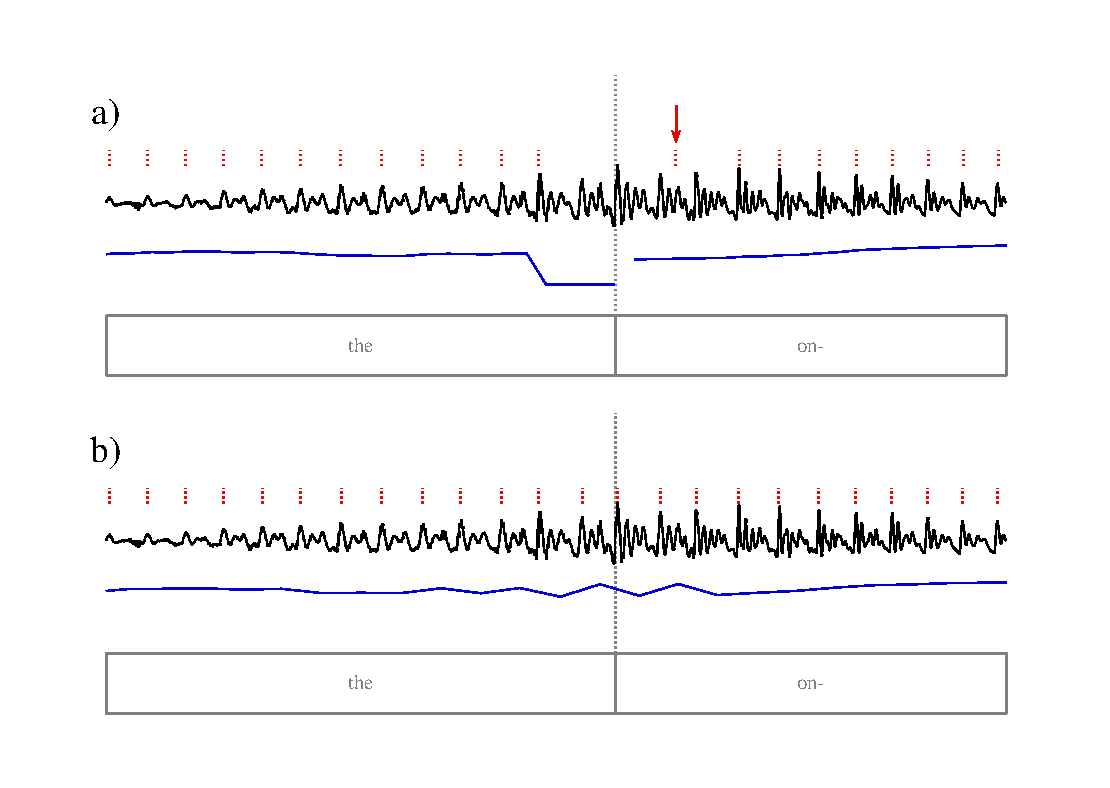
\includegraphics{figures/creakJitterShimmer/creakJitterShimmer.eps}
	\caption[Handling of creaky voicing in resynthesis]{Illustration of method for handling creaky-voiced portions of speech.  (a)~Excerpt of Talker~\ac{b}’s recording of sentence 33–05, in which vowel hiatus is resolved with light creaky voicing.  The waveform (black) is overlaid with Praat’s auto-detected pulse marks (dotted red lines) and pitch track (dashed blue line).  Note the missed cycles on either side of the red arrow, and the phase-shift of all pulses right of the arrow.  (b)~The same span of speech after manual correction of pulses, and a (jittery, but continuous) pitch track generated from the corrected pulses.\label{fig:JitShim}}
	\end{centering}
\end{figure}

%\subsection{Intensity}
Intensity was altered by first multiplying the signal by the difference of the maximum intensity and the inverted intensity contour (see Figure~\ref{fig:IntenManip}), then multiplying the resulting signal by the intensity contour of the replacement prosody and scaling as needed to achieve the desired \ac{rms} amplitude.  To do this, the donor intensity contour first underwent dynamic time warping to match the durational patterns of the target signal (see Script~\ref{scr:Psola}).

\begin{figure}
	\begin{centering}
	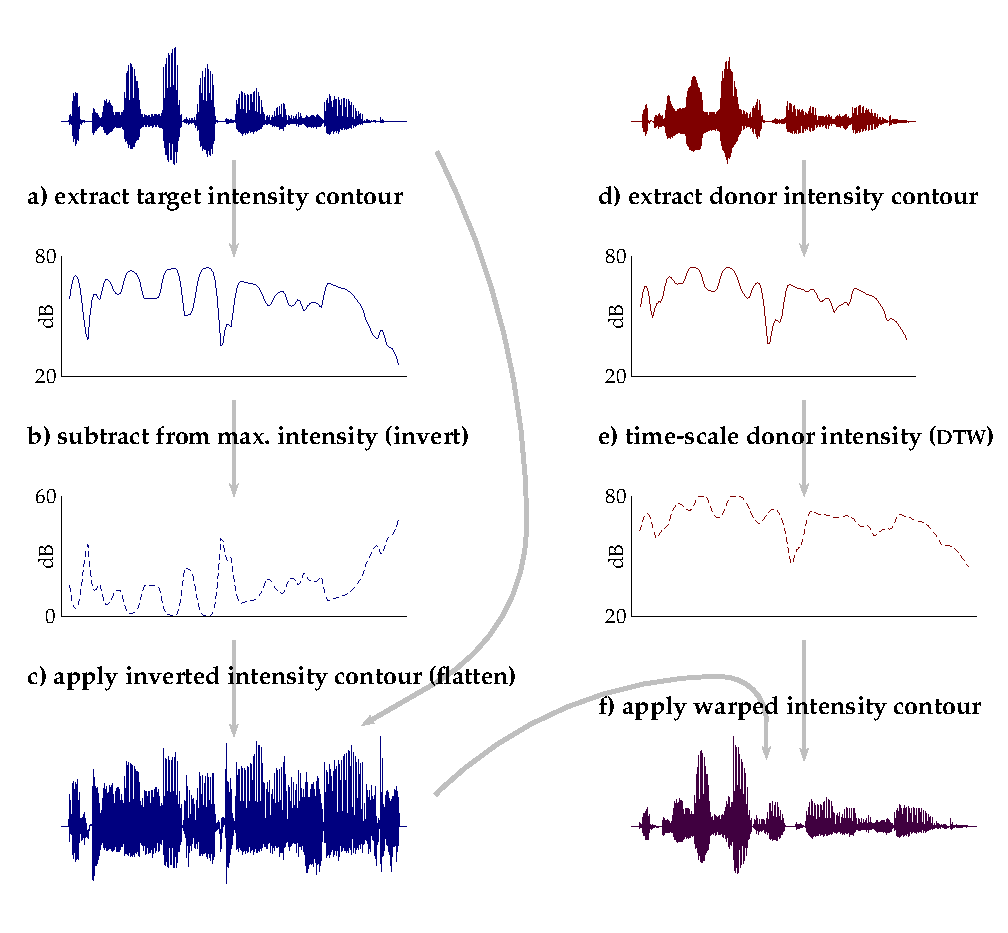
\includegraphics{figures/intensity/intensity2.eps}
	\caption[Intensity scaling in resynthesis]{Illustration of the method used to scale intensity.  (a)~Intensity contour is extracted from target waveform (blue).  (b)~The intensity contour of the target signal is inverted, by subtracting each intensity point from the maximum intensity.  (c)~Target intensity is \term{neutralized} or \term{flattened} by multiplying the target signal by the inverted intensity contour.  (d)~Intensity contour is extracted from the prosodic donor signal (red).  (e)~The prosodic donor intensity contour is time-scaled syllable-by-syllable via dynamic time warping (\ac{dtw}) to match the temporal pattern of the target signal.  (f)~The intensity-neutralized target signal is multiplied by the time-warped donor intensity contour (purple).  The signal is now ready for \psola{} resynthesis of duration and pitch.\label{fig:IntenManip}}
	\end{centering}
\end{figure}

%\subsection{}
After resynthesis, all stimuli were assessed auditorily for excessive distortion.  In some cases, problems could be remedied by readjusting the pulses and pitch tracks, and re-running the resynthesis script; in other cases the problems were irremediable, and the unacceptable donor\slsh{}target\slsh{}sentence combination was excluded from the experimental stimuli.  Most cases of irremediable stimuli arose from one of two sources: intra-syllable segment duration and intensity mismatches (see Figure~\ref{fig:SegDurMismatch}), or complete devoicing of a syllable by the target talker (see Figure~\ref{fig:Devoicing}).

\begin{figure}
	\begin{centering}
	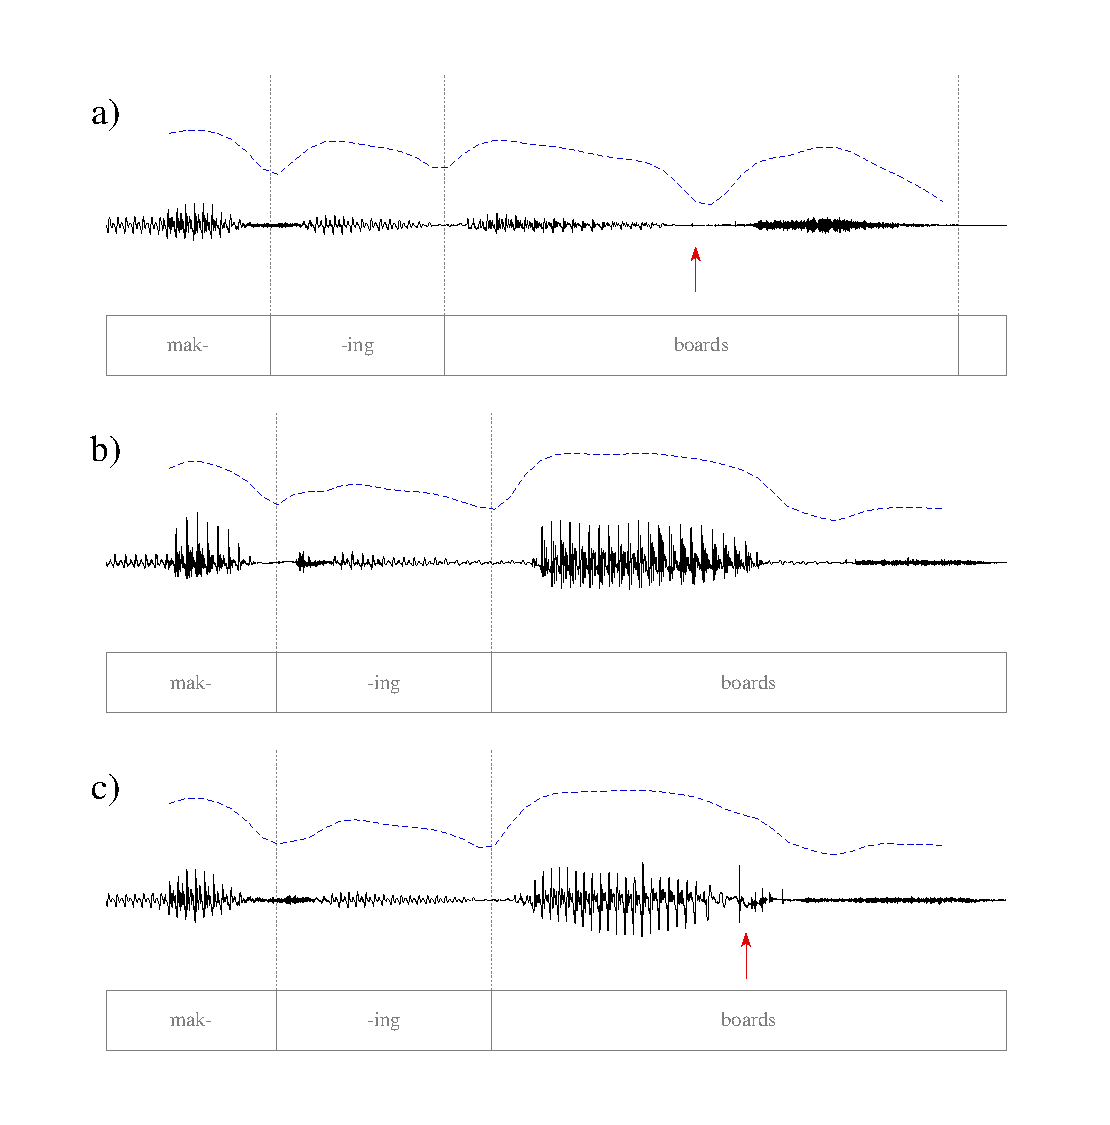
\includegraphics{figures/segmentMismatch/segmentMismatch.eps}
	\caption[Segment duration mismatch in resynthesis]{Illustration of intra-syllable segment duration and intensity mismatch, which led to unnatural patterns of intensity after resynthesis.  (a)~Waveform (black line) of Talker~\ac{c}’s pronunciation of “boards” in sentence 06–05, overlaid with intensity contour (blue dashed line).  Note that the syllable duration is split roughly 50/50 between the periodic nucleus and the aperiodic coda.  (b)~Talker~\ac{a}’s recording of the same sentence.  Note the relatively longer vocalic nucleus and relatively shorter coda.  (c)~Talker~\ac{c}’s waveform after resynthesis to match Talker~\ac{a}’s intensity, pitch, and duration.  The red arrow marks a nearly silent portion of Talker~\ac{c}’s speech that was amplified to vowel-like intensity levels.\label{fig:SegDurMismatch}}
	\end{centering}
\end{figure}

\begin{figure}
	\begin{centering}
	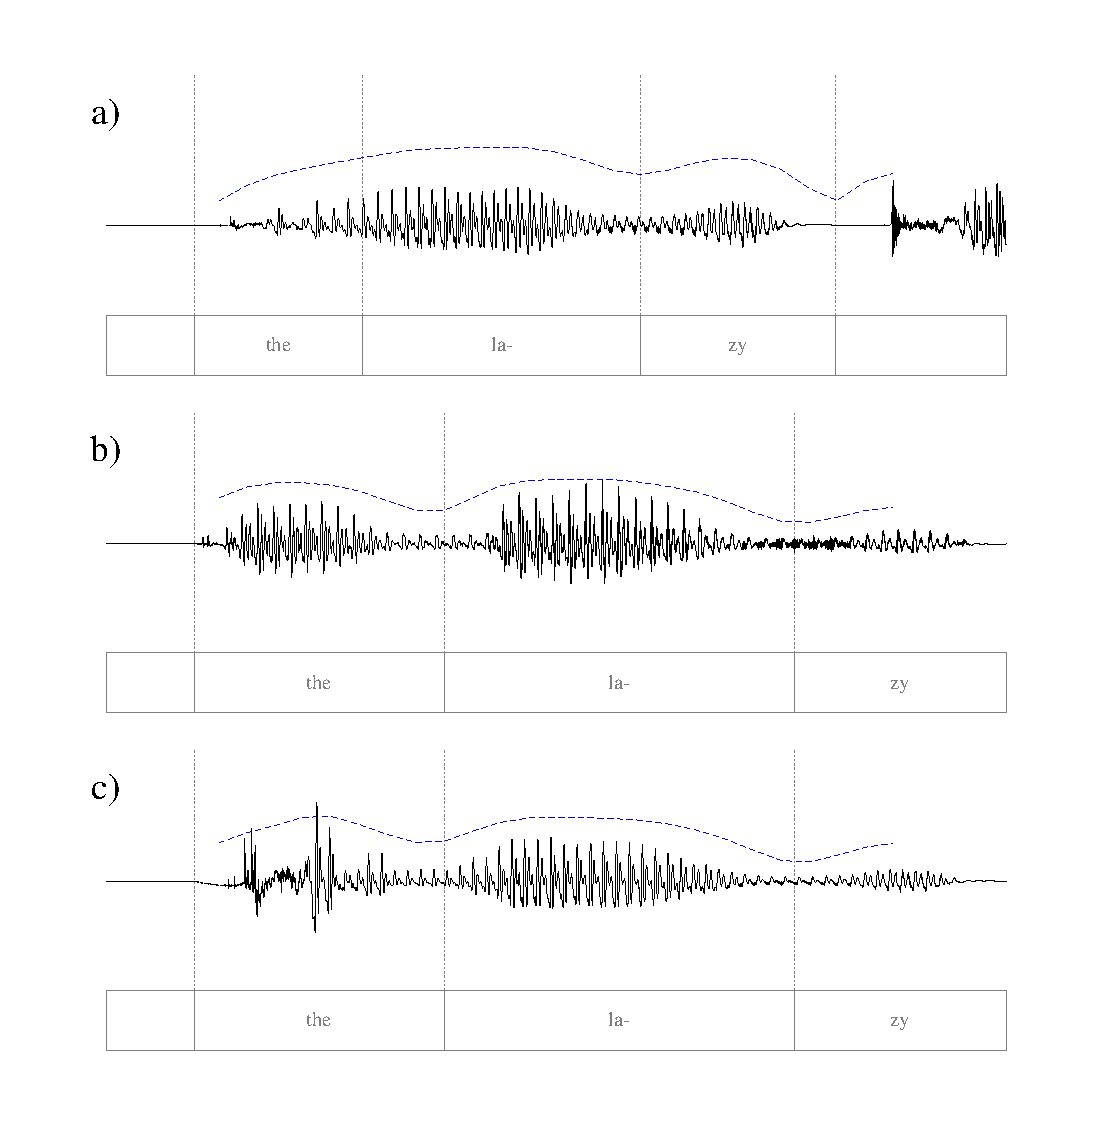
\includegraphics{figures/devoicing/devoicing.eps}
	\caption[Syllable devoicing in resynthesis]{Illustration of how devoicing can lead to unacceptable levels of distortion during resynthesis.  (a) Devoicing of the word “the” in Talker~\ac{b}’s recording of sentence 05–05 (first ≈500 ms shown).  The intensity contour (blue dashed line) is overlaid on the waveform (black).  (b) Talker~\ac{a}’s recording of the same sentence.  (c) Talker~\ac{b}’s waveform after resynthesis to match Talker~\ac{a}’s intensity, pitch, and duration.  Note the excessively high amplitude in the first syllable.\label{fig:Devoicing}}
	\end{centering}
\end{figure}

\section{Experiment sessions}
% Rationale for how much training to do:  
% \citep{YonanSommers2000}: Trained talkerID on 4 talkers (2M2F) over 2 days.  Each day: 60 exposure trials, 40 trials training w/ feedback, 60 more exp, 40 more training, 80 test.  All phases were half high-context and half low-context sentences.  End of day 2: single words \& sentences in SNR -5,0,+5, half high- half low-context, half familiar talkers half novel, half male talkers half female.  Familiar/unfamiliar talkers were piloted to make sure they were equally intelligible generally, and to old vs young people.  RESULTS: young listeners near ceiling on talkerID both day1 and day2; old listeners 73\% and 76\%.  Training on sentence material did not aid on the single word task (same as NygaardPisoni1998).  There was a benefit of familiar talker for sentence materials, which was stronger at lower SNRs.  A similar pattern obtained for a second experiment with talker exposure instead of talkerID training.
% \citep{VanEngen2012}: Two 30-minute training sessions (64 sentences) with noise (either SSN, English 2-babble, Mandarin 2-babble) and feedback.  Posttest 1 familiar, 1 unfamiliar talker, half in English babble, half in mandarin.  Trained and tested at their HINT threshold -3dB (based on VanEngen2010) to avoid floor/ceiling.  Results: “(1) listeners were able to take advantage of target talker familiarity; (2) training with babble was more effective than SSN training; and (3) after babble training, listeners improved most in coping with the babble in which they were trained [English or Mandarin]. In general, the results show that processes related both to tuning in to speech targets and tuning out speech maskers can be improved with auditory training”

Except where otherwise noted, stimuli were presented with a stationary Gaussian masker noise, frequency shaped to match the long term spectral average of the corpus of stimuli, at 0 dB \ac{snr}.  This \ac{snr} was chosen to avoid ceiling and floor effects, based on a pilot study testing five \ac{snr}s ranging from −1 to +3 dB.  To ensure target audibility, the level of the speech was held constant at 67 dB \ac{spl} (dB \ac{rms} in a 6 cc coupler) and the masker noise was digitally added to the speech to achieve the desired \ac{snr}, yielding a final presentation level of approximately 70 dB \ac{spl}.  The noise extended past the beginning and end of the speech by 50 ms in each direction, and linear onset and offset ramps were applied to this excess noise to prevent clicks during stimulus playback.

The combined speech-and-noise signal was presented in a sound-insulated booth over closed-back supra-aural headphones (Sennheiser HD 25–1 II).  Listeners were instructed to repeat each sentence they heard, to give partial answers when they only heard some words, and to guess when they were unsure.  Trials were scored 0–5 on keywords correct during the task.  An audio recording was made of listener responses, and scoring uncertainties were resolved offline.  

Of the 180 sentences in the corpus, half were set aside for use as training\slsh{}exposure sentences in Experiment~2; the remaining 90 sentences were designated as test sentences and resythesized versions of those sentences were created.  Experiment~1 presented the 90 test sentences to each listener, with equal numbers of stimuli from each “talker” (\ie, ten from each of the three unmodified talkers \ac{a}, \ac{b}, and \ac{c}, plus ten from each of the six resynthesized “talkers” \ac{ab}, \ac{ac}, \ac{ba}, \ac{bc}, \ac{ca}, and \ac{cb}).  Talker-sentence combinations were random and unique for each listener, subject to the above-mentioned constraints (\ie, each listener heard each talker an equal number of times, and each listener heard each sentence only once).

In Experiment~2, the 90 training sentences were presented in speech-shaped noise at 0 dB \ac{snr}.  After each listener had finished responding, the sentence was played again without background noise, and the text of the sentence was simultaneously presented on a computer screen for the listener to read.  For each listener, all 90 training sentences were recordings of the same talker, but the test sentences were again drawn in equal numbers from among the three unmodified talkers (\ac{a}, \ac{b}, and \ac{c}) and the six resynthesized “talkers” (\ac{ab}, \ac{ac}, \ac{ba}, \ac{bc}, \ac{ca}, and \ac{cb}).

\section{Participants}
Listeners were all native English speakers who lived in the Pacific Northwest (Washington, Oregon, or Idaho) throughout their period of primary and secondary education (\ie, ages 6–18).  All reported English as the primary home language, and all had learned or studied at least one other language as an adolescent or adult (though this was not a criterion for inclusion).  All listeners had bilaterally normal hearing, defined as pure-tone thresholds of 20 dB \ac{hl} or better at octave intervals from 250 Hz to 8 kHz \citepalias[re:][]{ansi2004}.  Listeners were recruited from the UW campus community and were compensated for their participation; there were 17 listeners in Experiment~1, and XXX listeners in Experiment~2.  One participant was excluded from Experiment~1 due to a mild monaural threshold elevation at 8 kHz.  Listener demographics are summarized in Table~\ref{tab:ListDemo}.

\begin{table}
	\caption[Listener demographics]{Listener demographics for Experiments~1 and~2.  Experiment~2a represents the listener group trained on Talker~\ac{c}; Experiment~2b represents the listener group trained on a talker not among the test talkers.\label{tab:ListDemo}}
	\centering
	\begin{tabu} to 0.6\textwidth {llX[2]XXX}
		\toprule
		\rowfont{\bfseries} & & & \multicolumn{3}{c}{Experiment}\\
		\rowfont{\bfseries} & & & 1 & 2a & 2b\\
		\midrule
		\textbf{Gender} & Female & & 8 & 0 & 0\\
		                & Male   & & 8 & 0 & 0\\
		\midrule
		\textbf{Age} & mean      & & 22.3 & 0 & 0\\
		             & st.\ dev. & &  6.9 & 0 & 0\\
		             & min.      & & 18   & 0 & 0\\
		             & max.      & & 44   & 0 & 0\\
		\taburulecolor{ltgray}
%		\midrule
%		Ethnicity & & & \\
		\taburulecolor{black}
		\bottomrule
	\end{tabu}
\end{table}

\section{Data analysis}
Data were analyzed using {\inlinecode R} \citep{R}, in particular the packages {\inlinecode lme4} for mixed-effects regression \citep{lmer} and {\inlinecode languageR} for calculating p-values for mixed-effects regression coefficients using Markov-chain Monte Carlo methods \citep{languageR}.  \comment{I’ll say more here when I know exactly which post-hoc tests I end up doing.}

\chapter{Results\label{chap:Results}}
This chapter describes the results of the two experiments conducted for this thesis.  Statistical models and post\-/hoc acoustic analyses that help to clarify and explain the results are also presented.

\section{Experiment 1}
Experiment~1 tests the role of prosody in intelligibility, by comparing mean sentence scores for unmodified talkers against resynthesized stimuli with prosodic replacement.  A quartile analysis indicated a significant improvement in performance between the first and last quartiles (\textit{t}=−3.016 on 709.3 degrees of freedom, \textit{p}<0.01; see Figure~\ref{fig:ExpOneQuartile}).  The magnitude of the difference between the first and fourth quartiles is approximately 0.4 keywords.

\begin{figure}[bt]
	\begin{centering}
	\includegraphics{figures/results/ExpOneQuartileBarplot.eps}
	\caption[Mean sentence scores by quartile for Experiment~1]{Mean sentence scores by quartile for Experiment~1.  Error bars are ±1 standard error.\label{fig:ExpOneQuartile}}
	\end{centering}
\end{figure}

The mean sentence score for each talker across listeners is shown in Figure~\ref{fig:ExpOneBarplot}.  Darker bars indicate unmodified stimuli, while light bars represent resynthesized stimuli.  It is noteworthy that not all resynthesized stimuli have lower mean scores compared to their unmodified counterparts, suggesting that distortion due to the resynthesis process was relatively minimal.  This is likely due to several factors; one is probably the painstaking hand\-/correction of the pulse marks during stimulus preparation, which ensured consistent phase of the \fo{} epochs throughout voiced spans of speech.  Another possible explanation for the low levels of distortion is the choice to maintain each talker’s natural mean pitch on each sentence, and map only the {\emph shape} of the pitch contour of the prosodic donor during resynthesis.  

With regard to Research Question~1 — \emph{how does prosody relate to intelligibility?} — a complex picture emerges.  Talker~\ac{b} suffers dramatically when his prosody is replaced, whereas Talker~\ac{c} is unchanged or slightly improved, and Talker~\ac{a} is unchanged or slightly worsened.  One possible explanation for these results is to postulate that Talker~\ac{a}, despite being highly intelligible, does not have especially good prosody, evidenced in particular by the fact that scores for Talker~\ac{ca} are lower than the scores for Talker~\ac{cb}.  On the same grounds, and on the additional observation that scores for Talker~\ac{ab} are greater than for Talker~\ac{ac}, we might conclude that Talker~\ac{b} has more intelligible prosody than the other two talkers, and his middling base intelligibility scores are due to segmental factors.

\begin{figure}[bt]
	\begin{centering}
	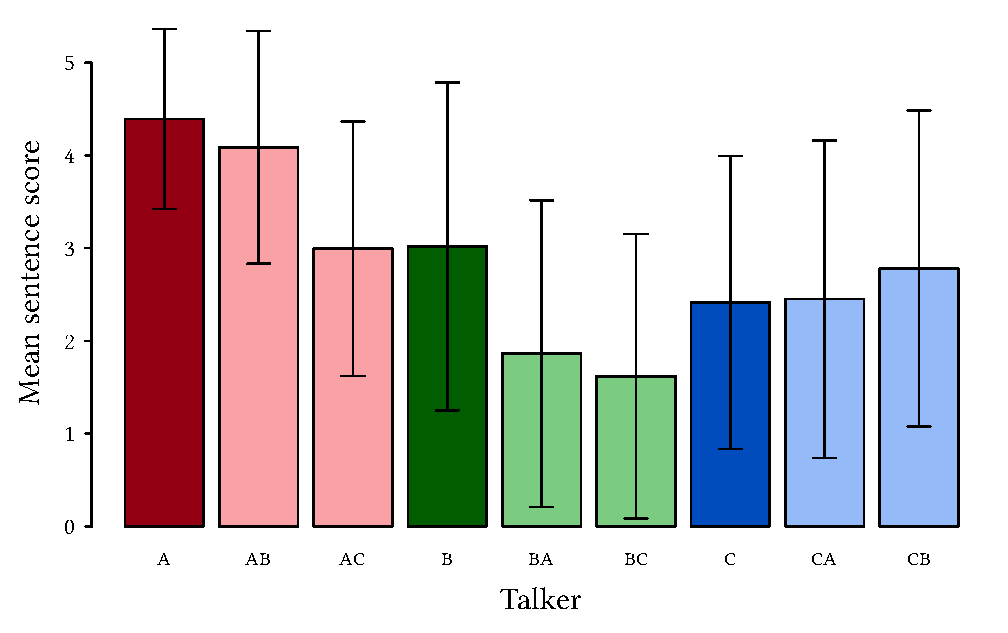
\includegraphics{figures/results/ExpOneBarplot.eps}
	\caption[Barplot of mean sentence scores for Experiment~1]{Barplot of mean sentence scores for Experiment~1.  Error bars are ±1 standard error; lighter colors indicate resynthesized talkers, with the second letter indicating the prosodic donor (see Section~\ref{sec:ExpDesign} for full explanation of talker codes).  Similar hues indicate shared segmental donors.\label{fig:ExpOneBarplot}}
	\end{centering}
\end{figure}

With regard to the question of whether low\-/intelligibility talkers can be made more intelligible through prosody alone, it would appear that the answer is “yes”: Talker~\ac{cb} appears to have higher scores than Talker~\ac{c}, despite the likelihood that Talker~\ac{cb}’s recordings suffer some amount of distortion from the resynthesis process, however small.  In other words, any degradation due to resynthesis seems to have been more than overcome by the benefit of having Talker~\ac{b}’s prosody mapped onto Talker~\ac{c}’s signal.  However, it is noteworthy that the greatest improvement to Talker~\ac{c}’s intelligibility does not come from Talker~\ac{a}’s prosody, even though Talker~\ac{a} has the highest overall intelligibility.  This suggests that hihg\-/intelligibility talkers do not necessarily use prosody that enhances their intelligibility.

\subsection{Experiment~1 statistical model}
To further probe these results, the scores were submitted to a mixed\-/effects linear regression model, shown here:%in Equation~\ref{eq:ExpOneMM}:

\noindent{\small\inlinecode lmer(sentScore\textasciitilde resynth+segDonor+proDonor+trial+(1|listener)+(1|sentence))}
%\begin{equation}\label{eq:ExpOneMM}
%	\text{{\small \inlinecode lmer(sentScore\textasciitilde resynth+segDonor+proDonor+(1|listener)+(1|sentence), data=allData)}}
%\end{equation}

In this model, the dependent variable {\inlinecode sentScore} is the number of keywords correct (0–5), and is being predicted by several independent variables: {\inlinecode resynth} is a Boolean variable that is true for Talkers~\ac{ab}, \ac{ac}, \ac{ba}, \ac{bc}, \ac{ca} and~\ac{cb}, and {\inlinecode segDonor} and {\inlinecode proDonor} are three\-/level factors indicating the talker in the target signal and the talker from whom the prosodic information was drawn, respectively.  For the unmodified original recordings, {\inlinecode segDonor} and {\inlinecode proDonor} are defined as the talker himself, even though those recordings were not resynthesized.  The effect of task familiarization seen in Figure~\ref{fig:ExpOneQuartile} is accounted for by the fixed\-/effect predictor {\inlinecode trial} (a numeric value ranging from 1–90).  Two random\-/effects predictors ({\inlinecode 1|listener} and {\inlinecode 1|sentence}) are also included to model variability in listener performance and sentence difficulty, respectively. 

%A summary of the model shown in Equation~\ref{eq:ExpOneMM} 
A summary of fixed\-/effects predictors for this model is given in Table~\ref{tab:ExpOneFixedEff}.  All fixed\-/effects predictors were significantly different from zero, and there was no evidence of correlation of fixed effects (correlation coefficients all less than 0.1; not shown).  The baseline condition is Talker~\ac{a}, with a value at the intercept of about 4.1 words correct.  The coefficients reveal similar patterns to those seen in Figure~\ref{fig:ExpOneBarplot}: firstly, the model supports the interpretation that Talker~\ac{b} has the most intelligible prosody.  Having the prosody of Talker~\ac{b} represents a net gain of 0.3 words correct over the prosody of Talker~\ac{a}, whereas having the prosody of Talker~\ac{c} represents a net loss of more than 0.6 words correct compared to Talker~\ac{a}.  The model also supports the idea that Talker~\ac{a}’s intelligibility stems in large part from non\=/prosodic factors, given that the other levels of {\inlinecode segDonor} both have strongly negative coefficients.  The estimated degradation due to resynthesis is about −0.7 keywords correct.  Because trial was a continuous variable ranging from 1–90, the coefficient for the effect of trial is misleadingly small; the predicted difference between the first and the last trial due to listener adaptation to the task is actually 90×0.005549, or 0.5 keywords.

\begin{table}[tbp]
	\caption[Experiment~1 statistical model: Fixed effects]{Summary of fixed effect predictors in the statistical model of Experiment~1.  \textit{s}: standard error of the coefficient estimate; \textit{t}: \textit{t}\=/value of coefficient estimate; \textit{p}: \textit{p}\=/value of coefficient estimate (calculated via \ac{mcmc}).\label{tab:ExpOneFixedEff}}
	\centering
	\begin{tabu} spread 1em {Xrcrc}
		\toprule
		\multicolumn{5}{l}{Summary of fixed effects (N=1440; log-likelihood=−2551)}\\
		\rowfont\bfseries
		\multicolumn{1}{l}{Predictor} & \multicolumn{1}{c}{Coefficient} & \textit{s} & \multicolumn{1}{c}{\itshape t} & \textit{p}\\
		\midrule
		Intercept         &  4.132 & (0.145) &  28.44 & <10⁻¹⁶\\
		resynth = TRUE    & −0.662 & (0.077) &  −8.63 & <10⁻¹⁶\\
		segDonor = \ac{b} & −1.673 & (0.089) & −18.86 & <10⁻¹⁶\\
		segDonor = \ac{c} & −1.278 & (0.089) & −14.31 & <10⁻¹⁶\\
		proDonor = \ac{b} &  0.307 & (0.088) &   3.48 & <10⁻³\\
		proDonor = \ac{c} & −0.646 & (0.088) &  −7.36 & <10⁻¹²\\
		trial             &  0.006 & (0.001) &   4.02 & <10⁻⁴\\
		\bottomrule
	\end{tabu}
\end{table}

A summary of the random effects in the model for Experiment~1 are shown in Table~\ref{tab:ExpOneRandomEff}.  The results here are not unexpected: the variance in intercepts due to particular listeners doing systematically better or worse on the task is only about 2\% of the total residual variance.  This suggests that, by and large, all listeners were performing equally well on the task.  The variance in intercepts due to varying difficulty of particular sentences is somewhat larger (about 22\% of the total residual variance, or a standard deviation of 0.7 keywords correct),\footnotemark{} suggesting that there was indeed some value in modeling the sentences as varying in their difficulty (cf. the discussion of scoring in Section~\ref{sec:Scoring}).
\footnotetext{The \ac{mcmc} estimate for variability due to listener is in close agreement with the fitted model.  The \ac{mcmc} estimate for variability due to sentence is slightly smaller than the value in the fitted model, at 16\% of the total variance (\vs\ 22\%), with a standard deviation for sentence of about 0.6 keywords (\vs\ 0.7).}

\begin{table}[tbp]
	\caption[Experiment~1 statistical model: Random effects]{Summary of random effects in the statistical model of Experiment~1.  \textit{s}²: estimated variance; \textit{s}: standard error; \ac{hpd}: highest posterior density interval.\label{tab:ExpOneRandomEff}}
	\centering
	\begin{tabu} spread 1em {Xcccc}
		\toprule
		\multicolumn{3}{l}{Summary of random effects} & \multicolumn{2}{c}{\bfseries \ac{mcmc} (nsim=10\thinspace000)}\\ 
		\cmidrule{4-5}
		\rowfont\bfseries
		Group & \textit{s}² & \textit{s} & mean & 95\% \ac{hpd}\\
		\midrule
		Sentence (intercept) & 0.506 & 0.711 & 0.600 & (0.498~~0.700)\\
		Listener (intercept) & 0.043 & 0.207 & 0.220 & (0.100~~0.346)\\
		Residual             & 1.767 & 1.329 & 1.344 & (1.294~~1.396)\\
		\bottomrule
	\end{tabu}
\end{table}

\section{Experiment 2}
Experiment~2 tests the role of prosody in the familiar talker advantage, by comparing mean sentence scores for various talkers across two groups of listeners: those trained on one of the test talkers (Talker~\ac{c}), and those trained on a control talker (Talker~\ac{d}).  The first question to be addressed is whether the training phase was in fact effective for both groups of listeners.   

\begin{figure}[bt]
	\begin{centering}
	\includegraphics{figures/results/ExpTwoOctileBarplot.eps}
	\caption[Quartile analysis of Experiment~2 training and testing phases]{Quartile analysis of training and testing phases in Experiment~2 (all listeners combined).  Significant improvement is seen during the training phase, but not during testing.\label{fig:ExpTwoOctileBarplot}}
	\end{centering}
\end{figure}

Across all listeners, performance shows an upward trend in mean sentence score across training quartiles (\textit{t}=−4.00 on 878.3 degrees of freedom, \textit{p}<0.0001), but no significant changes across quartiles of the testing phase (see Figure~\ref{fig:ExpTwoOctileBarplot}).  This suggests that training was successful in general, and that any familiarization effects were complete before the start of the testing phase.

Considering the control and experimental listener groups separately, both show an upward trend in mean sentence score across training quartiles, and \textit{t}\=/tests performed on the first and fourth quartile of each group show a statistically significant improvement in both groups of listeners (control group: \textit{t}=−2.898 on 437.2 degrees of freedom, \textit{p}<0.01; experimental group: \textit{t}=−2.816 on 438.1 degrees of freedom, \textit{p}<0.01; see Figure~\ref{fig:Quartile}).  The magnitude of the improvement differs slightly between the control group (0.50 keywords) and the experimental group (0.38 keywords).  

\begin{figure}[bt]
	\begin{centering}
	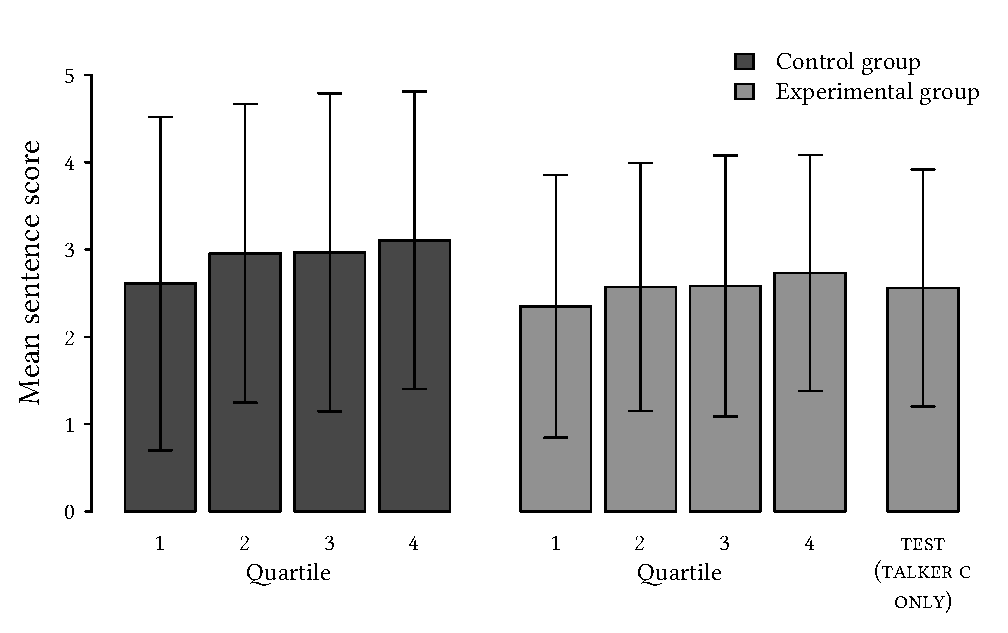
\includegraphics{figures/results/QuartileBarplot.eps}
	\caption[Quartile analysis of Experiment~2 training phase by group]{Quartile analysis of training phase in Experiment~2.  Improvement is seen during training for both the control group (trained on Talker~\ac{d}) and the experimental group (trained on Talker~\ac{c}).  The adaptation in the experimental group appears not to have persisted through the testing phase.\label{fig:Quartile}}
	\end{centering}
\end{figure}

For the experimental group, it appears that familiarization with Talker~\ac{c} during training did not confer an advantage on Talker~\ac{c} during testing (compare the last quartile of the training phase to the score on Talker~\ac{c} during the testing phase in Figure~\ref{fig:Quartile}).  %\footnotemark{}
%\footnotetext{This is true at least for the listeners trained on Talker~\ac{c}.  Listeners trained on Talker~\ac{d} did not hear their training talker during the testing phase, so it is unknown whether any adaptation was retained during testing.  Presumably, however, any such adaptation would have had little effect on performance when listening to Talkers~\ac{a}, \ac{b}, or \ac{c}.}
In light of this, it is perhaps unsurprising that training did not confer a reliable perceptual advantage on test stimuli resynthesized to have the training talker’s prosody; this is seen in the barplot of mean sentence scores for the testing phase of Experiment~2 (Figure~\ref{fig:ExpTwoBarplot}).  Even without controlling for multiple comparisons, none of the \textit{t}\=/tests comparing the experimental and control groups within talker are significant, suggesting that there was no familiar talker advantage enjoyed by the experimental group.  If there had been a familiar talker advantage, we would have expected the colored bars to be higher than their corresponding grey bars for Talker~\ac{c}, and perhaps for Talkers~\ac{ca}, \ac{cb}, \ac{ac} and \ac{bc} (depending on whether and how the advantage extended to resynthesized talkers).

\begin{figure}[bt]
	\begin{centering}
	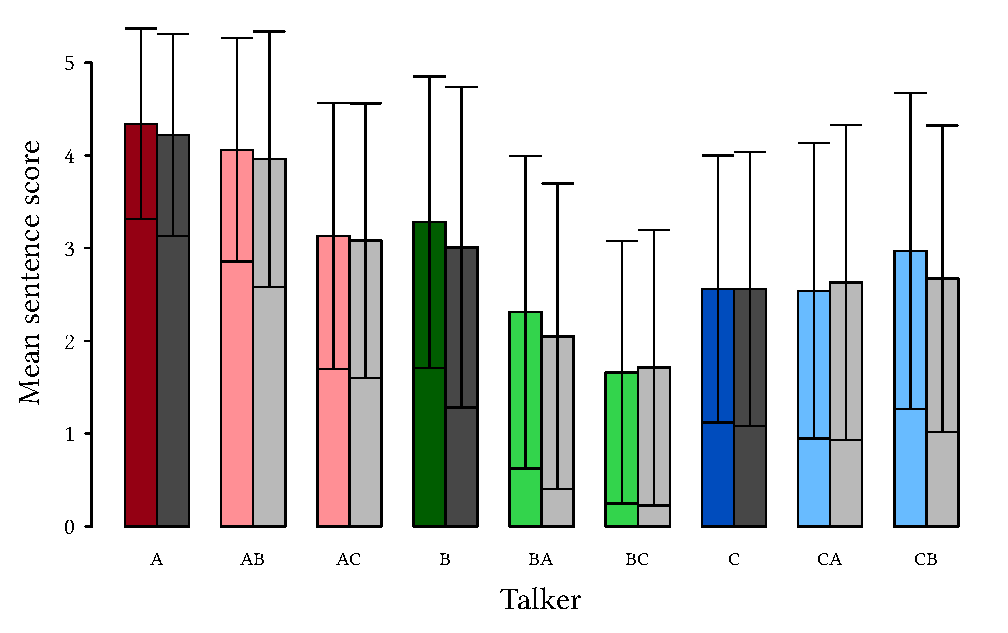
\includegraphics{figures/results/ExpTwoBarplot.eps}
	\caption[Barplot of mean sentence scores for Experiment~2]{Barplot of mean sentence scores for Experiment~2.  Error bars are ±1 standard error.  Colored bars indicate the experimental group; grayscale bars the control group.  Lighter colors indicate resynthesized talkers, and similar hues indicate shared segmental donors.\label{fig:ExpTwoBarplot}}
	\end{centering}
\end{figure}

\subsection{Experiment~2 statistical model}
Full results of the statistical model for Experiment~2 are shown in Table~\ref{tab:ExpTwoFixedEff}.  Predictor codes are the same as in the model for Experiment~1, with the addition of Boolean variables {\inlinecode segTrain} (indicating match between the training talker and the segmental donor of the test stimulus) and {\inlinecode proTrain} (indicating match between the training talker and the prosodic donor of the test stimulus).  

\begin{table}[tbp]
	\caption[Experiment~2 statistical model: Fixed effects]{Summary of fixed effect predictors in the statistical model of Experiment~2.  \textit{s}: standard error of the coefficient estimate; \textit{t}: \textit{t}\=/value of coefficient estimate; \textit{p}: \textit{p}\=/value of coefficient estimate (calculated via \ac{mcmc}).\label{tab:ExpTwoFixedEff}}
	\centering
	\begin{tabu} spread 1em {Xrcrc}
		\toprule
		\multicolumn{5}{l}{Summary of fixed effects (N=1800; log-likelihood=−3103)}\\
		\rowfont\bfseries
		\multicolumn{1}{l}{Predictor} & \multicolumn{1}{c}{Coefficient} & \textit{s} & \multicolumn{1}{c}{\itshape t} & \textit{p}\\
		\midrule
		Intercept	         &  4.366 & (0.139) &  31.50 & <10⁻¹⁶\\
		resynth = \ac{true}  & −0.603 & (0.066) &  −9.15 & <10⁻¹⁶\\
		segDonor = \ac{b}    & −1.466 & (0.075) & −19.42 & <10⁻¹⁶\\
		segDonor = \ac{c}    & −1.159 & (0.098) & −11.80 & <10⁻¹⁶\\
		proDonor = \ac{b}    &  0.270 & (0.075) &   3.60 & <10⁻³\\
		proDonor = \ac{c}    & −0.584 & (0.098) &  −5.95 & <10⁻⁸\\
		segTrain = \ac{true} &  0.008 & (0.125) &   0.06 & 0.95\\
		proTrain = \ac{true} & −0.117 & (0.125) &  −0.94 & 0.35\\
		trial                & −0.001 & (0.001) &  −0.64 & 0.53\\
		\bottomrule
	\end{tabu}
\end{table}

Unlike the model for Experiment~1, there is no significant effect for {\inlinecode trial} (unsurprising given Figure~\ref{fig:ExpTwoOctileBarplot}), most likely because listeners had already undergone a training phase and were already familiarized to the task.  Niether of the two new predictors {\inlinecode segTrain} and {\inlinecode proTrain} were significant, suggesting that listeners were not realizing a familiarity advantage due to training.  Aside from the lack of effect for {\inlinecode trial} and the two additional non\=/significant predictors {\inlinecode segTrain} and {\inlinecode proTrain}, the model is nearly identical to the model for Experiment~1; the magnitude, direction, and significance of the other fixed\-/effect predictors are all unchanged from Experiment~1.

A summary of the random effects in the model of Experiment~2 are shown in Table~\ref{tab:ExpTwoRandomEff}.  The results are also very similar to Experiment~1, with estimates of listener accounting for about 4\% of the total unexplained variability (with a standard deviation of 0.3 keywords) and sentence accounting for about 24\% of total unexplained variability (with a standard deviation of about 0.7 keywords).\footnotemark{}

\footnotetext{Again, \ac{mcmc} estimates for the effect of sentence were slightly smaller than the fitted model (18\% \vs\ 24\%), and there was close agreement between the two for the effect of listener.}

\begin{table}[tbp]
	\caption[Experiment~2 statistical model: Random effects]{Summary of random effects in the statistical model of Experiment~2.  \textit{s}²: estimated variance; \textit{s}: standard error; \ac{hpd}: highest posterior density interval.\label{tab:ExpTwoRandomEff}}
	\centering
	\begin{tabu} spread 1em {Xcccc}
		\toprule
		\multicolumn{3}{l}{Summary of random effects} & \multicolumn{2}{c}{\bfseries \ac{mcmc} (nsim=10\thinspace000)}\\ 
		\cmidrule{4-5}
		\rowfont\bfseries
		Group & \textit{s}² & \textit{s} & mean & 95\% \ac{hpd}\\
		\midrule
		Sentence (intercept) & 0.537 & 0.733 & 0.617 & (0.526~~0.712)\\
		Listener (intercept) & 0.083 & 0.288 & 0.297 & (0.192~~0.425)\\
		Residual             & 1.617 & 1.271 & 1.285 & (1.242~~1.329)\\
		\bottomrule
	\end{tabu}
\end{table}

\section{\Ph{} acoustic analyses}
Overall, the statistical models for Experiments~1 and~2 support the view that both prosodic and non\=/prosodic factors contribute to differences in the intelligibility of talkers.  To better understand these results, a variety of acoustic measurements were performed on the stimuli, in hopes of identifying the acoustic dimensions that underlie the effects seen in the statistical models.  The measures are broadly divided into segmental measures (presence of stop release bursts, properties of the vowel space) and prosodic measures (mean pitch range, pitch velocity, pitch dynamicity, intensity velocity, intensity dynamicity, and syllable duration).

\subsection{Segmental measures}
The results of the stop consonant reduction analysis are shown in Figure~\ref{fig:ReleaseBursts}.  The percentages given are calculated as the total number of stops and affricates counted (across the 45 sentences measured) divided by the total number of expected stop consonants based on citation\-/form phonemic transcriptions; there was little difference between this method and the method of calculating the mean of unreduced stop percentage calculated on a per-stimulus basis.  The relative ordering of the talkers accords with their relative intelligibility (\ie, Talker~\ac{a}~> Talker~\ac{b}~> Talker~\ac{c}), but does not correspond to the expected ordering based on coefficients for segmental donor (\ac{a}~> \ac{c}~> \ac{b}).  

\begin{figure}[bt]
	\begin{centering}
	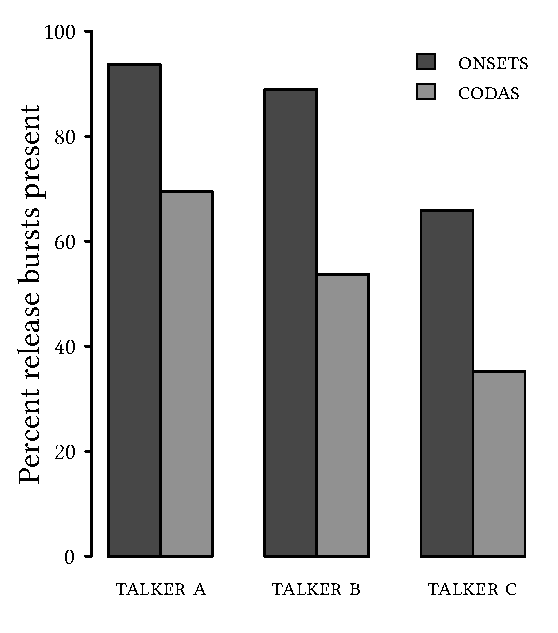
\includegraphics{figures/posthocs/ReleaseBursts.eps}
	\caption[Barplot of mean proportion of unreduced stop consonants]{Barplot of mean proportion of unreduced stop consonants present, calculated across half of the test stimuli (45 sentences per talker).\label{fig:ReleaseBursts}}
	\end{centering}
\end{figure}

A possible explanation for the ordering of talkers is that stop reduction may index both segmental and prosodic information, for two reasons: first, stop consonants often occur at word edges, which are loci for word\-/level prosodic marking, and second, stop consonants are often strengthened in prosodically prominent syllables at higher levels of phrasal structure (cf., \eg, \citealt{deJong1995, FougeronKeating1997, ChoEtAl2007, ColeEtAl2007}; see \citealt{Keating2006} for review).  In other words, because stop consonant reduction was measured across all words in the sentence, it may reflect a combination of each talker’s prosodic habits (\ie, tendency toward more \vs\ fewer intonational phrases) as well as purely segmental pronunciation habits (which might have been more easily observed from words lists).  Unfortunately, the \ac{pn/nc} corpus does not include recordings of word lists, so this explanation must remain speculative.

Results of the \ph{} analysis of vowel space size is shown in Figure~\ref{fig:VowelSpace}.  Here the expected pattern of \ac{a}~> \ac{c}~> \ac{b} (based on coefficients for segmental donor from Experiments~1 and~2) is seen in three of the five measures: mean distance from center, area of the convex hull, and F1 range.  F2 range does not correlate with any expected intelligibility-related pattern, while area of the polygon based on vowel means seems to correlate with overall intelligibility scores for each talker (\ie, \ac{a}~> \ac{b}~> \ac{c}).  

\begin{figure}[bt]
	\begin{centering}
	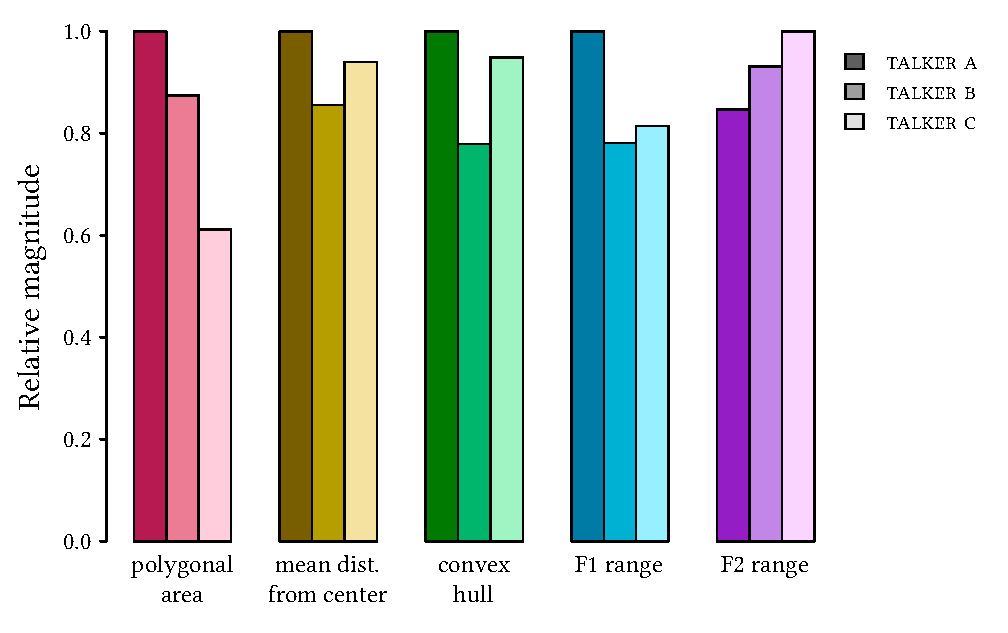
\includegraphics{figures/posthocs/VowelSpace.eps}
	\caption[Barplot of vowel space size metrics]{Barplot of the relative magnitudes of several vowel space size metrics.  Each metric has been scaled by dividing by the maximum value among the three talkers.\label{fig:VowelSpace}}
	\end{centering}
\end{figure}

The difference between area of the convex hull and area of the vowel means polygon is especially interesting.  Figure~\ref{fig:ConvexHull} plots both the convex hull and vowel means polygons on data from Talker~\ac{a}.  This figure illustrates one possible explanation for the difference in patterning between these two measures of vowel space size: the convex hull effectively ignores vowel tokens that are reduced (for any reason) — and thus indexes a talker’s most extreme vowel productions — whereas the area of the vowel means polygon includes information from multiple vowel tokens, which may show reduction due to prosodic differences between talkers (because the tokens came from various positions within the sentence).  Considering that all the vowel tokens measured came from lexically stressed syllables in content words, any vowel quality reduction present in these tokens is \emph{not} reduction due to lack of \emph{lexical} stress; thus it is quite likely that the reduction seen is prosodic in origin.

\begin{figure}[bt]
	\begin{centering}
	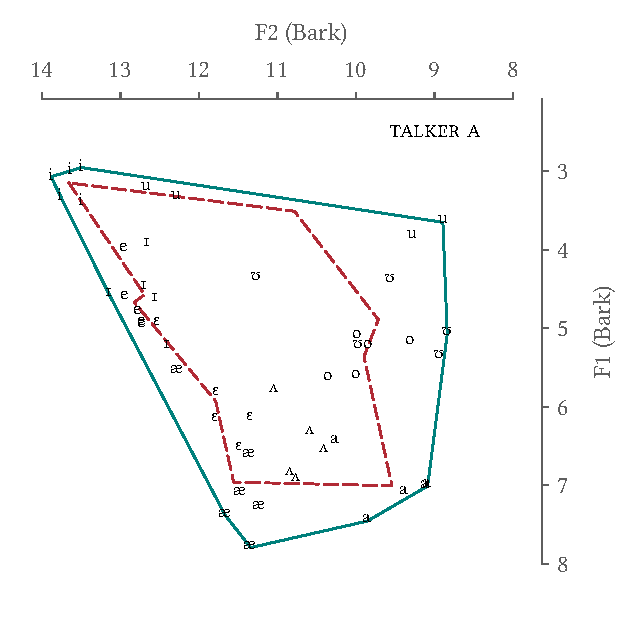
\includegraphics{figures/posthocs/ConvexHull.eps}
	\caption[Vowel space metrics]{Illustration of two vowel space area metrics (data from Talker~\ac{a}).  The area of the polygon described by vowel means (dashed red line) is contrasted with the convex polygonal hull (solid blue line).  Note the difference between the polygons in the high\-/back and low\-/front regions due to /u/-fronting and /æ/-raising (respectively), as well as differences due to reduction (particularly in the /o/, /ʊ/ and /ɛ/ regions).\label{fig:ConvexHull}}
	\end{centering}
\end{figure}

The distribution of vowel tokens in Figure~\ref{fig:ConvexHull} raises another issue regarding vowel space size, which is that information about vowel category overlap and within\-/category variation — both potentially relevant factors to intelligibility — are not reflected in measures of convex hull area, but are somewhat conflated with the area of the vowel means polygon.  For example, the large variation in F2 of the high back vowel /u/ drastically reduces the area of the vowel means polygon when compared to the convex hull, but the variation in /u/ is likely not due to reduction, but rather is an example of the widespread change\-/in\-/progress known as /u/-fronting \citep[chap.\ 12]{LabovEtAl2006}.  Similar variation is seen in F1 values for /æ/ (cf. reports of /æ/-raising before velars in the Pacific Northwest: \citealt{Reed1952, WassinkEtAl2009}).  In this way, area of the vowel means polygon could be said to contain information about both segmental and prosodic dimensions of speech (much like stop consonant reduction discussed above), and may explain why it corresponds to the ordering of talkers based on general intelligibility scores, rather than the ordering of talkers based on segmental donor coefficients in the statistical models.  In contrast, area of the convex hull may be a better index of purely segmental properties of speech, since it ignores within-category variation of vowels (at least some of which is prosodically\-/motivated); this would explain why area of the convex hull correlates with the ordering of talkers based on signal donor coefficients.

These examples suggest a need to disentangle overall vowel space expansion from individual vowel category size, and to include measures of category overlap or encroachment.  Measures of mean cluster size and repulsive force of each talker’s vowel system are shown in Figure~\ref{fig:ForceCluster} (see Section~\ref{sec:SegmentalMethods} for definition of these measures).

\begin{figure}[bt]
	\begin{centering}
	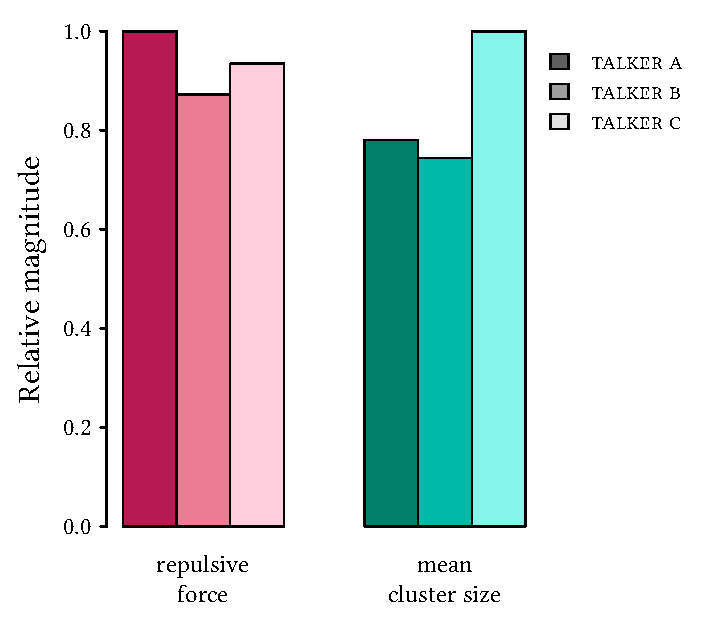
\includegraphics{figures/posthocs/ForceCluster.eps}
	\caption[Barplot of vowel overlap and encroachment metrics]{Barplot of the relative magnitudes of mean vowel cluster size and repulsive force.  Each metric has been scaled by dividing by the maximum value among the three talkers.\label{fig:ForceCluster}}
	\end{centering}
\end{figure}

A high degree of repulsive force indexes a high degree of phonemic overlap, which ought to correspond to \emph{lower} intelligibility (on the assumption that words would be more confusible in talkers whose phonemic categories are not well segregated).  Thus the expected pattern based on the statistical model coefficients for segmental donor ought to be \ac{b}~> \ac{c}~> \ac{a}, which is precisely the opposite of the pattern seen in Figure~\ref{fig:ForceCluster}.  It is possible that fifty vowel tokens (five per vowel) was simply not enough to give an accurate picture of the internal structure of the vowel space.  In any case, the likelihood of lexical confusion due to vowel phoneme overlap is contingent on the existence and lexical probability of the competing form.  For example, no matter how much /u/-fronting a talker exhibits, the /u/ vowel in “poodles” (sentence 15–06) is unlikely to be heard as /i/.  Duration is also relevant: although “kits” and “Kate’s” are potentially confusable based on formant values (see Talker~\ac{a}’s vowel plot in Figure~\ref{fig:ConvexHull}), there are likely to be duration differences that listeners can rely on to disambiguate.  Thus it is unsurprising that repulsive force is a poor predictor in a sentence perception task such as this one (as opposed to an isolated word perception task in which stimuli are chosen to ensure the viability of competing forms, and plausibility is not constrained by semantic context).

Mean cluster size should index within\-/category variability of vowel formants, and is predicted (like repulsive force) to be inversely correlated with the non\-/prosodic component of intelligibility.  However, like repulsive force, the magnitudes of mean cluster size also fail to track the expected pattern of \ac{b}~> \ac{c}~> \ac{a}.  Again, a possible explanation is that an insufficient number of vowel tokens were available to give accurate estimates of the spectral extent of within\-/category variation.  Another explanation is that because mean cluster size collapses information across vowels, it does not distinguish differences in crowded parts of the vowel space from differences in sparse regions.  This suggests the need for a hybrid measure somehow encompassing both within\-/category variation and category overlap or encroachment.  More research is needed to determine how such a measure could be calculated.

\subsection{Prosodic measures}
\begin{figure}[bt]
	\begin{centering}
	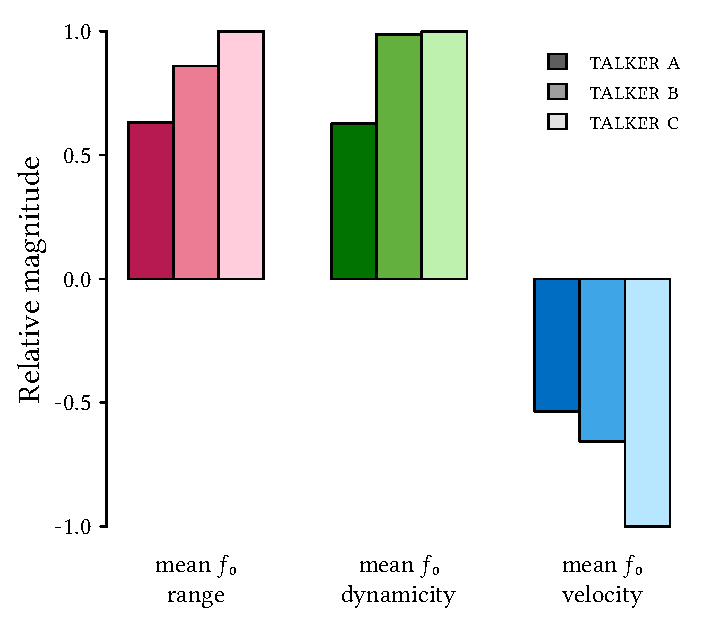
\includegraphics{figures/posthocs/ProsodicMeasuresPitchOnly.eps}
	\caption[Barplot of \fo{} metrics]{Barplot of the relative magnitudes of three \fo-related metrics.  Each metric has been scaled by dividing by the maximum absolute value among the three talkers.\label{fig:ProsodicMeasuresPitch}}
	\end{centering}
\end{figure}

\Ph{} analyses of the prosodic measures related to \fo{} are shown in Figure~\ref{fig:ProsodicMeasuresPitch}.  The expected pattern based on statistical model coefficients for prosodic donor is Talker~\ac{b}~> Talker~\ac{a}~> Talker~\ac{c}.  None of the three measures match this pattern exactly; the closest is mean \fo{} dynamicity, which shows a pattern of \ac{b}~≈ \ac{c}~> \ac{a}.  Mean \fo{} range shows a pattern of \ac{c}~> \ac{b}~> \ac{a}, as does mean \fo{} velocity (in the case of velocity, “>” meaning “more negative”).\footnotemark{}  One explanation that ties these three measures together is the fact that Talker~\ac{c} exhibits a lot of creaky voicing in his speech, especially utterance\-/finally, which accounts for his highly negative value of \fo{} velocity (nearly twice the magnitude of Talker~\ac{a}).  The relatively frequent occurrence of creaky voicing in Talker~\ac{c}’s stimulus sentences can be seen in Figure~\ref{fig:PitchTracks}, by the high number of “tails” protruding downward from the main mass of pitch tracks at the ends of several sentences.
\footnotetext{Recall that dynamicity is a measure of the mean of the \emph{absolute value} in rate of change of \fo, whereas velocity is the mean of the signed rate of change.  As such, velocity reflects overall trends in pitch across the utterance, whereas dynamicity better indexes the magnitude of pitch movements throughout the utterance.}

\begin{figure}[pbt]
	\begin{centering}
	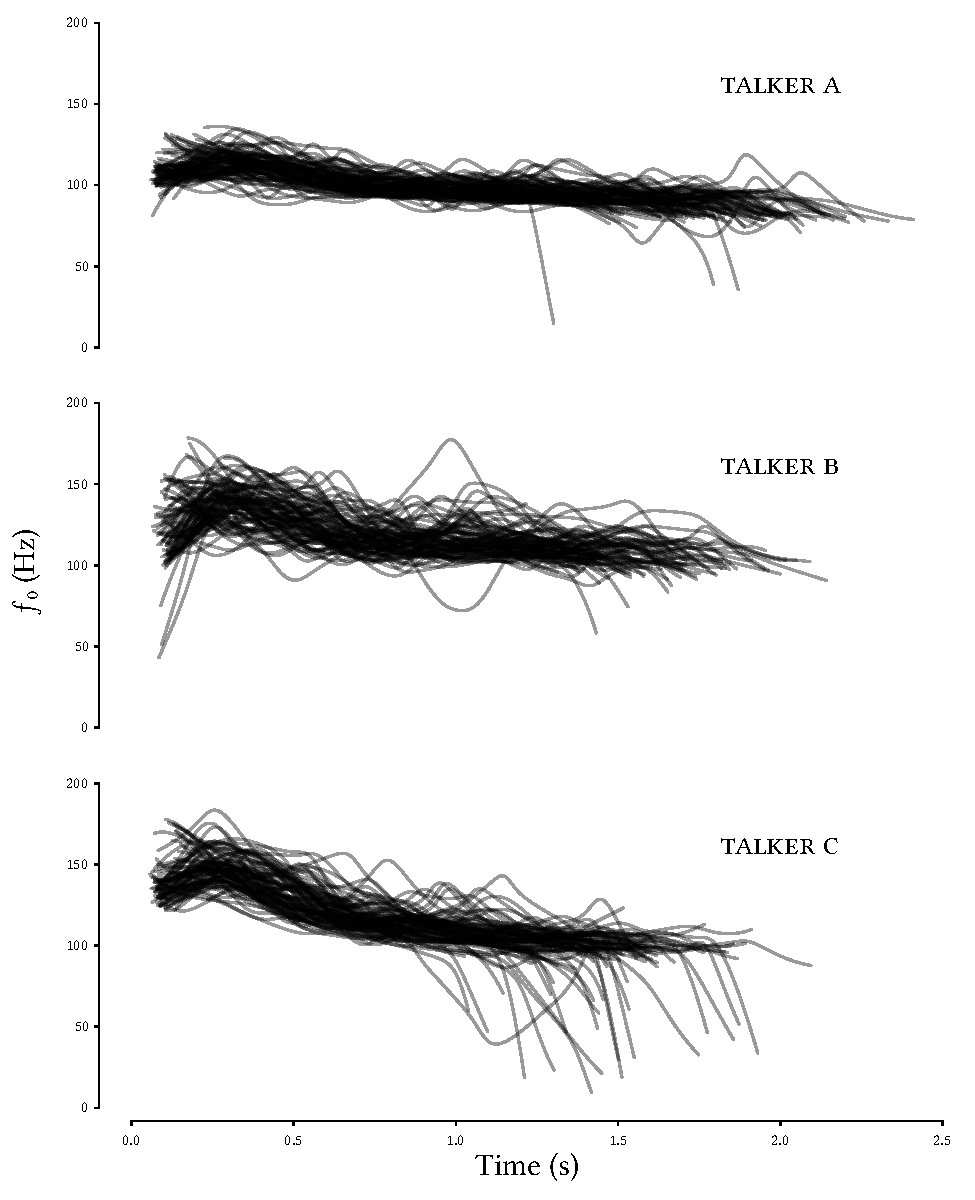
\includegraphics{figures/posthocs/PitchTracks.pdf}
	\caption[Pitch track overlays of the test sentences]{Overlaid pitch tracks for Talkers~\ac{a}, \ac{b} and~\ac{c} for the 90 test sentences.  Pitch tracks have been smoothed by fitting a local polynomial weighted by a Gaussian kernel with a bandwidth of 75 ms.  Note the frequent occurrence of utterance\-/final creaky voicing (indicated by extreme drops in \fo) for Talker~\ac{c}.\label{fig:PitchTracks}}
	\end{centering}
\end{figure}

The consistent use of creaky voicing also inflates Talker~\ac{c}’s values for mean \fo{} range and mean \fo{} dynamicity.  Re\=/examining Figure~\ref{fig:ProsodicMeasuresPitch} in this light, we see that both mean \fo{} range and mean \fo{} dynamicity show the expected relationship between Talkers~\ac{a} and~\ac{b}.  Figure~\ref{fig:PitchTracks} also visually illustrates Talker~\ac{a}’s low \fo{} range (the tighter clustering of his pitch tracks compared to Talker~\ac{b}) and dynamicity (the straightness of the lines in his pitch tracks compared to Talker~\ac{b}).

\begin{figure}[bt]
	\begin{centering}
	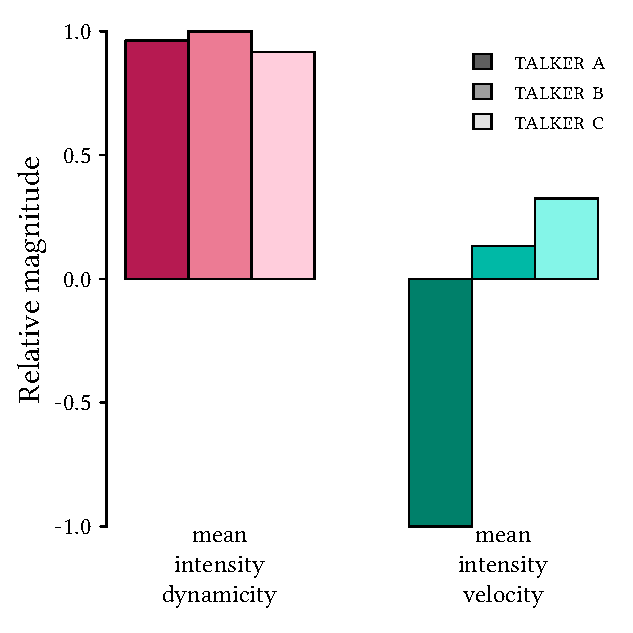
\includegraphics{figures/posthocs/ProsodicMeasuresIntensityOnly.eps}
	\caption[Barplot of intensity metrics]{Barplot of the relative magnitudes of two intensity-related metrics.  Each metric has been scaled by dividing by the maximum absolute value among the three talkers.\label{fig:ProsodicMeasuresIntensity}}
	\end{centering}
\end{figure}

\Ph{} analyses of the prosodic measures related to intensity are seen in Figure~\ref{fig:ProsodicMeasuresIntensity}.  The values for mean intensity dynamicity follow the predicted pattern of \ac{b}~> \ac{a}~> \ac{c}, but only the difference between Talkers~\ac{b} and~\ac{c} is significant.  The small differences between talkers is probably due to the fact that intensity dynamicity mostly tracks something like obstruent\slsh sonorant alternation rate, since the largest\-/magnitude intensity modulations in speech (at all but the shortest time scales) are the inherent differences between segment types — voiceless stop closures at one extreme, and open vowels at the other (cf. the well\-/known linguistic notion of \term{sonority}).  Because all talkers read the same set of sentences, the patterns of obstruent\-/sonorant alternation were by and large identical across talkers (modulo variation due to segmental reduction) and therefore any variation due to inter\-/talker differences in prosody are likely to be relatively small in comparison (and thus hard to detect statistically).

\begin{figure}[pbt]
	\begin{centering}
	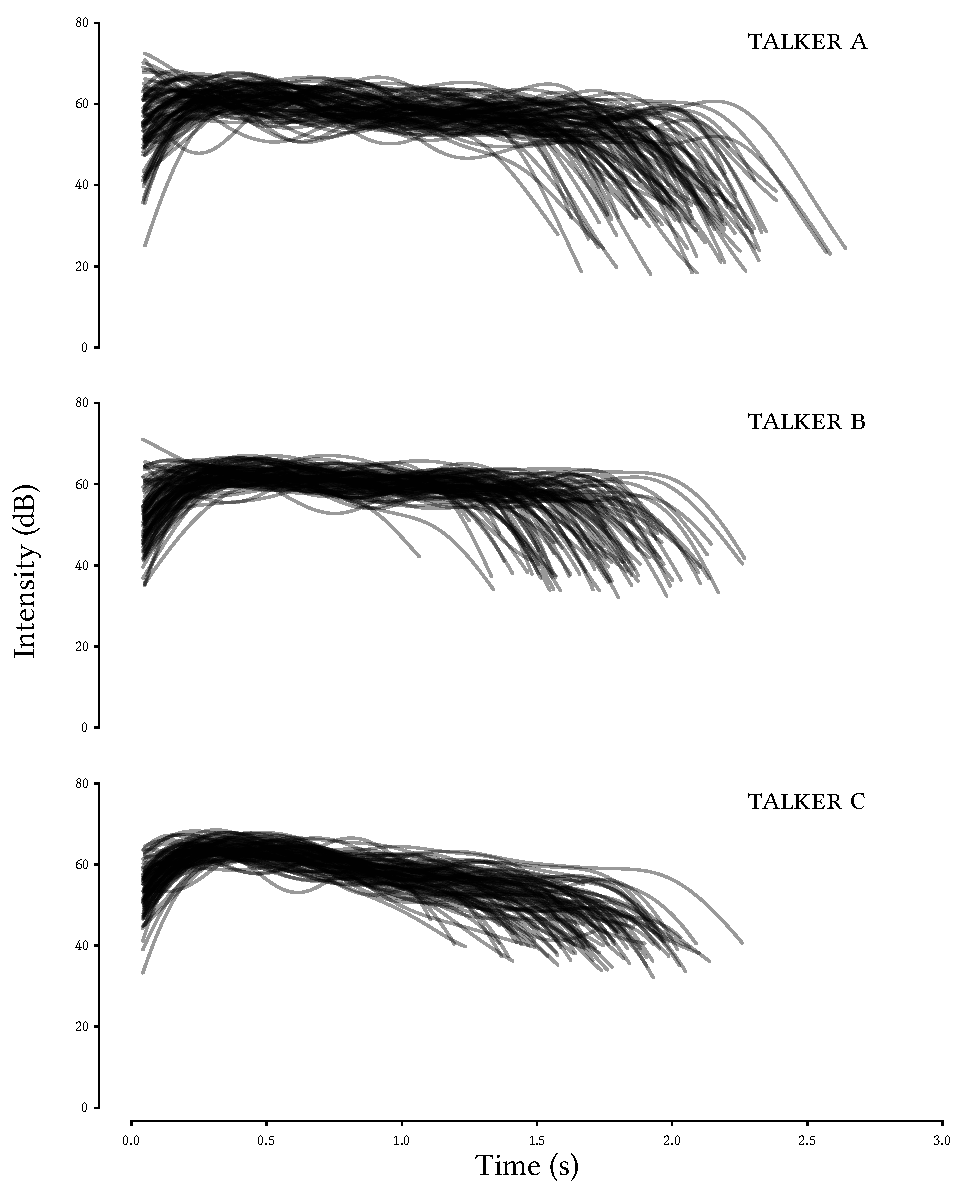
\includegraphics{figures/posthocs/IntensityTracks.pdf}
	\caption[Intensity track overlays of the test sentences]{Overlaid pitch tracks for Talkers~\ac{a}, \ac{b} and~\ac{c} for the 90 test sentences.  Pitch tracks have been heavily smoothed by fitting a local polynomial weighted by a Gaussian kernel with a bandwidth of 150 ms.\label{fig:IntensityTracks}}
	\end{centering}
\end{figure}

Values for mean intensity velocity show an unusual pattern in which Talker~\ac{a} shows an extreme negative value, with Talkers~\ac{b} and~\ac{c} showing small positive values (see Figure~\ref{fig:ProsodicMeasuresIntensity}).  Some insight into this pattern is available if we examine the overlaid intensity tracks for each talker, as seen in Figure~\ref{fig:IntensityTracks}.  At the expense of showing detail at smaller time scales, the wide (150~ms) smoothing bandwidth highlights the overall trends in intensity in each recording, and reveals the strong intensity drop\=/off at the end of most of Talker~\ac{a}’s sentences, the smaller drop\=/off in Talker~\ac{b}’s speech, and the tendency for Talker~\ac{c}’s speech to decline more gradually in intensity across the sentence.  The strong drop\=/off is responsible for Talker~\ac{a}’s large negative value for mean intensity velocity seen in Figure~\ref{fig:ProsodicMeasuresIntensity}; in fact, given that mean intensity velocity is anticorrelated with talker intelligibility, we can infer that the strong drop\=/off is probably less damaging to the intelligibility of speech in noise than a gradual decline.  This makes sense if Talker~\ac{a}’s tendency for utterance\-/final drop\=/off likely only affects the last word, whereas Talker~\ac{c}’s tendency for more gradual intensity decline gradually reduces \ac{snr} for words occurring mid\=/sentence.

\begin{figure}[bt]
	\begin{centering}
	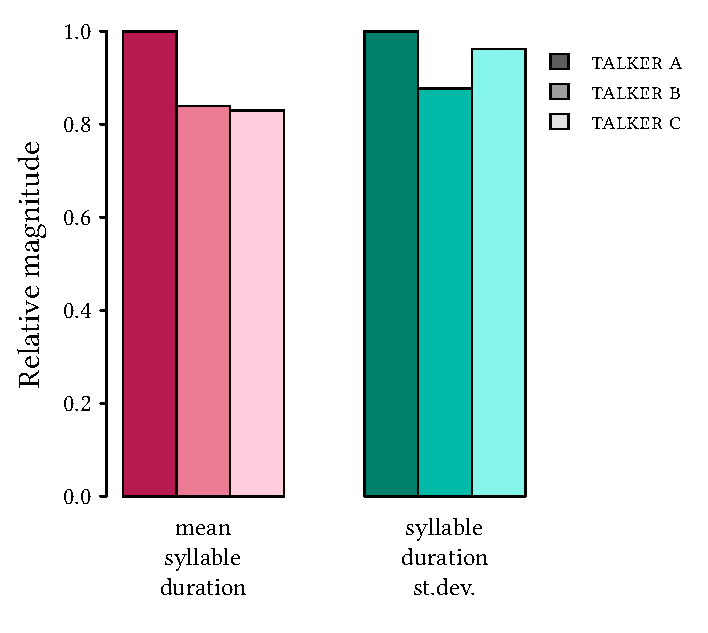
\includegraphics{figures/posthocs/SyllableDuration.eps}
	\caption[Barplot of duration metrics]{Barplot of the relative magnitudes of two duration-related metrics.  Each metric has been scaled by dividing by the maximum absolute value among the three talkers.\label{fig:SyllableDuration}}
	\end{centering}
\end{figure}

\Ph{} analyses of syllable duration are seen in Figure~\ref{fig:SyllableDuration}.  Mean syllable duration for Talkers~\ac{b} and~\ac{c} is nearly identical, and thus cannot explain the difference in intelligibility between them.  This is consistent with findings in the literature suggesting that within\-/talker changes in intelligibility are not necessarily accompanied by a change in speech rate \citep{KrauseBraida2002}; further interpretation of mean speech rate values is limited by the small number of talkers investigated here.  Interestingly, \emph{variability} in syllable duration appears to follow the pattern of non\=/prosodic coefficients (\ie, \ac{a}~> \ac{c}~> \ac{b}).  This is unexpected, since large variability in syllable duration is expected to index more extreme duration contrasts between prominent and reduced syllables (more a prosodic phenomenon than a segmental or lexical one).  This result also merits further investigation with a larger sample of talkers.

% \subsection{\Ph{} statistical analysis}

\chapter{Discussion}

\section{Future directions}
\begin{itm}
	\item{decomposing effects of prosodic dimensions}
	\begin{itm}
		\item{{\bfseries Experiment 5:} What are the relative contributions of duration, pitch, and intensity to talker intelligibility?  (Repeat of experiment 1 where only 1 or 2 of the dimensions are replaced via resynthesis.)}
	\end{itm}
	\item{talker ID studies}
	\begin{itm}
		\item{{\bfseries Experiment 6:} Can you train listeners to make a reliable talker ID distinction on the basis of prosody alone?  Can listeners reliably categorize B/C and B/A as different talkers?}
		\item{{\bfseries Experiment 7:} Can you train listeners to make a reliable talker ID distinction when prosody has been neutralized?  Can listeners reliably categorize C/B and A/B as different talkers?}
	\end{itm}
\end{itm}


\end{spacing}

% BIBLIOGRAPHY (SINGLE SPACED)
\bibliographystyle{apa-good}
\bibliography{dissertation}

%\appendix
\titleformat{\chapter}{\LARGE\bfseries\doublespacing}{Appendix \thechapter.}{0.6em}{}
\begin{appendices}
\chapter{Stimulus sentences\label{apx:HarvardSents}}

\begin{longtabu} to 0.8\textwidth [c]{X[c] X[4]}
	% FIRST HEAD
	\caption[\ac{ieee} “Harvard” sentences used as stimuli]{\ac{ieee} “Harvard” sentences used as stimuli. Here “number” combines the “list” and “sentence” numbers from the original numeration given in \citet{HarvardSents}\label{tab:HarvardSents}}\\
	\toprule
	\rowfont[c]{\bfseries} Number & Text \\
	\midrule
	\endfirsthead

	% MAIN HEAD
	\caption[]{\ac{ieee} “Harvard” sentences used as stimuli {\itshape (continued from previous page)}}\\
	\midrule
	\rowfont[c]{\bfseries} Number & Text \\
	\midrule
	\endhead
	
	% MAIN FOOT
	\midrule 
	\multicolumn{2}{c}{\itshape continued on next page} \\
	\endfoot
	
	% LAST FOOT
	\bottomrule
	\endlastfoot

	01-07 & The box was thrown beside the parked truck. \\
	02-01 & The boy was there when the sun rose. \\
	02-06 & A pot of tea helps to pass the evening. \\
	03-10 & Read verse out loud for pleasure. \\
	04-02 & Take the winding path to reach the lake. \\
	04-04 & Wipe the grease off his dirty face. \\
	04-05 & Mend the coat before you go out. \\
	04-08 & The young girl gave no clear response. \\
	05-02 & The ship was torn apart on the sharp reef. \\
	05-05 & The lazy cow lay in the cool grass. \\
	05-07 & The rope will bind the seven books at once. \\
	06-01 & The frosty air passed through the coat. \\
	06-04 & The show was a flop from the very start. \\
	06-05 & A saw is a tool used for making boards. \\
	06-09 & Place a rosebush near the porch steps. \\
	06-10 & Both lost their lives in the raging storm. \\
	07-08 & This is a grand season for hikes on the road. \\
	07-09 & The dune rose from the edge of the water. \\
	07-10 & Those words were the cue for the actor to leave. \\
	08-04 & The walled town was seized without a fight. \\
	08-07 & The horn of the car woke the sleeping cop. \\
	10-06 & Bail the boat to stop it from sinking. \\
	10-09 & Ten pins were set in order. \\
	10-10 & The bill was paid every third week. \\
	11-05 & Add the sum to the product of these three. \\
	11-07 & The ripe taste of cheese improves with age. \\
	12-03 & The pennant waved when the wind blew. \\
	12-10 & We find joy in the simplest things. \\
	13-01 & Type out three lists of orders. \\
	13-03 & The boss ran the show with a watchful eye. \\
	13-07 & It caught its hind paw in a rusty trap. \\
	14-04 & Two plus seven is less than ten. \\
	14-06 & Bring your problems to the wise chief. \\
	15-06 & Pure bred poodles have curls. \\
	15-07 & The tree top waved in a graceful way. \\
	15-09 & Mud was spattered on the front of his white shirt. \\
	16-01 & The empty flask stood on the tin tray. \\
	16-02 & A speedy man can beat this track mark. \\
	17-03 & Drop the two when you add the figures. \\
	17-05 & An abrupt start does not win the prize. \\
	17-06 & Wood is best for making toys and blocks. \\
	18-01 & Steam hissed from the broken valve. \\
	18-02 & The child almost hurt the small dog. \\
	18-04 & The sky that morning was clear and bright blue. \\
	18-05 & Torn scraps littered the stone floor. \\
	18-06 & Sunday is the best part of the week. \\
	19-02 & Fairy tales should be fun to write. \\
	19-06 & Add the column and put the sum here. \\
	19-07 & We admire and love a good cook. \\
	19-10 & She has a smart way of wearing clothes. \\
	20-04 & The paper box is full of thumb tacks. \\
	22-01 & The cement had dried when he moved it. \\
	22-02 & The loss of the second ship was hard to take. \\
	22-03 & The fly made its way along the wall. \\
	22-04 & Do that with a wooden stick. \\
	22-06 & The large house had hot water taps. \\
	22-07 & It is hard to erase blue or red ink. \\
	23-01 & A pencil with black lead writes best. \\
	23-07 & The shaky barn fell with a loud crash. \\
	23-08 & Jazz and swing fans like fast music. \\
	23-09 & Rake the rubbish up and then burn it. \\
	24-02 & They are pushed back each time they attack. \\
	24-07 & Some ads serve to cheat buyers. \\
	24-09 & A waxed floor makes us lose balance. \\
	25-01 & On the islands the sea breeze is soft and mild. \\
	25-02 & The play began as soon as we sat down. \\
	25-04 & Add salt before you fry the egg. \\
	26-09 & These pills do less good than the others. \\
	27-06 & The rude laugh filled the empty room. \\
	27-07 & High seats are best for football fans. \\
	27-09 & A dash of pepper spoils beef stew. \\
	28-01 & The horse trotted around the field at a brisk pace. \\
	28-08 & The junk yard had a moldy smell. \\
	30-02 & The gold ring fits only a pierced ear. \\
	30-04 & Watch the log float in the wide river. \\
	30-06 & The heap of fallen leaves was set on fire. \\
	31-03 & The beam dropped down on the workman's head. \\
	31-04 & Pink clouds floated with the breeze. \\
	31-10 & The fight will end in just six minutes. \\
	32-09 & The purple tie was ten years old. \\
	33-01 & Fill the ink jar with sticky glue. \\
	33-05 & The crunch of feet in the snow was the only sound. \\
	33-08 & The plush chair leaned against the wall. \\
	34-01 & Nine rows of soldiers stood in line. \\
	34-02 & The beach is dry and shallow at low tide. \\
	34-05 & Pages bound in cloth make a book. \\
	34-06 & Try to trace the fine lines of the painting. \\
	34-08 & The zones merge in the central part of town. \\
	34-10 & Code is used when secrets are sent. \\
	36-01 & Pour the stew from the pot into the plate. \\
	36-08 & Our plans right now are hazy. \\
	36-10 & It takes a good trap to capture a bear. \\
	37-01 & Feed the white mouse some flower seeds. \\
	37-05 & Plead to the council to free the poor thief. \\
	37-09 & He crawled with care along the ledge. \\
	08-02 & The two men met while playing on the sand. \\
	16-10 & The sofa cushion is red and of light weight. \\
	22-08 & Write at once or you may forget it. \\
	31-01 & Slide the box into that empty space. \\
	38-02 & Mark the spot with a sign painted red. \\
	47-01 & The music played on while they talked. \\
	56-07 & A brown leather bag hung from its strap. \\
	65-03 & They sang the same tunes at each party. \\
	39-01 & He wrote down a long list of items. \\
	39-04 & Roads are paved with sticky tar. \\
	39-10 & The sun came up to light the eastern sky. \\
	40-06 & The desk was firm on the shaky floor. \\
	40-07 & It takes heat to bring out the odor. \\
	40-09 & Raise the sail and steer the ship northward. \\
	40-10 & A cone costs five cents on Mondays. \\
	41-02 & Jerk the dart from the cork target. \\
	41-08 & The sense of smell is better than that of touch. \\
	41-09 & No hardship seemed to keep him sad. \\
	42-09 & The point of the steel pen was bent and twisted. \\
	44-10 & The marsh will freeze when cold enough. \\
	45-01 & They slice the sausage thin with a knife. \\
	45-02 & The bloom of the rose lasts a few days. \\
	45-05 & Bottles hold four kinds of rum. \\
	45-08 & Drop the ashes on the worn old rug. \\
	45-10 & Throw out the used paper cup and plate. \\
	46-02 & The couch cover and hall drapes were blue. \\
	46-05 & The clothes dried on a thin wooden rack. \\
	47-04 & He sent the figs, but kept the ripe cherries. \\
	48-01 & The kite flew wildly in the high wind. \\
	48-03 & The tin box held priceless stones. \\
	49-05 & He offered proof in the form of a large chart. \\
	49-08 & They told wild tales to frighten him. \\
	50-01 & A man in a blue sweater sat at the desk. \\
	50-06 & Tuck the sheet under the edge of the mat. \\
	51-04 & The dusty bench stood by the stone wall. \\
	51-06 & Smile when you say nasty words. \\
	52-07 & The room was crowded with a wild mob. \\
	52-10 & The beetle droned in the hot June sun. \\
	53-01 & Press the pedal with your left foot. \\
	53-03 & The black trunk fell from the landing. \\
	53-09 & His wide grin earned many friends. \\
	55-01 & Those last words were a strong statement. \\
	55-02 & He wrote his name boldly at the top of the sheet. \\
	55-04 & Down that road is the way to the grain farmer. \\
	55-07 & If you mumble your speech will be lost. \\
	56-02 & Clams are small, round, soft, and tasty. \\
	56-08 & A toad and a frog are hard to tell apart. \\
	56-09 & A white silk jacket goes with any shoes. \\
	56-10 & A break in the dam almost caused a flood. \\
	57-02 & The child crawled into the dense grass. \\
	57-06 & A round hole was drilled through the thin board. \\
	57-09 & A vent near the edge brought in fresh air. \\
	58-03 & It was hidden from sight by a mass of leaves and shrubs. \\
	58-08 & The lobes of her ears were pierced to hold rings. \\
	59-04 & Drive the screw straight into the wood. \\
	59-05 & Keep the hatch tight and the watch constant. \\
	60-03 & Slide the tray across the glass top. \\
	60-07 & Dull stories make her laugh. \\
	60-09 & Get the trust fund to the bank early. \\
	60-10 & Choose between the high road and the low. \\
	61-09 & A six comes up more often than a ten. \\
	62-06 & The early phase of life moves fast. \\
	63-05 & She flaps her cape as she parades the street. \\
	64-05 & Crouch before you jump or miss the mark. \\
	64-06 & Pack the kits and don't forget the salt. \\
	65-08 & Pile the coal high in the shed corner. \\
	65-09 & A gold vase is both rare and costly. \\
	66-01 & The rarest spice comes from the far East. \\
	66-05 & The aim of the contest is to raise a great fund. \\
	67-01 & Hang tinsel from both branches. \\
	67-05 & Pick a card and slip it under the pack. \\
	67-06 & A round mat will cover the dull spot. \\
	67-09 & The mail comes in three batches per day. \\
	67-10 & You cannot brew tea in a cold pot. \\
	68-02 & Put the chart on the mantel and tack it down. \\
	68-08 & We don't like to admit our small faults. \\
	70-02 & It was a bad error on the part of the new judge. \\
	70-04 & Take the match and strike it against your shoe. \\
	70-06 & The baby puts his right foot in his mouth. \\
	70-09 & The streets are narrow and full of sharp turns. \\
	71-05 & The big red apple fell to the ground. \\
	71-06 & The curtain rose and the show was on. \\
	71-08 & He sent the boy on a short errand. \\
	72-05 & Small children came to see him. \\
	72-06 & The grass and bushes were wet with dew. \\
\end{longtabu}

\chapter{Praat scripts\label{apx:PraatScripts}}
% SCRIPT ORDER
% syllabic segmentation
% pitch settings/pulse correction
% psola
% create LTAS noise
% mix noise
% ramp edges

% SEGMENTATION
\section{Syllabic segmentation by intensity\label{scr:SyllIntens}}
This script takes a directory of sound files and, for each file, creates a new TextGrid and prepopulates an interval tier with boundaries at each local minimum of the sound file’s intensity contour.  It then presents the user with a TextGrid editor for the opportunity to adjust boundaries, add new ones, delete spurious ones, and add notes if desired.  The file name, notes (if any) and a sequential number are written to a log file.  Users can stop the script at any time, and resume work on the same directory of sound files by entering a “starting file number” when re-initiating the script.
\begin{code}
	\inputminted[fontsize=\footnotesize, tabsize=2]{r}{../scripts/dissversions/CreateSyllableTierFromIntensity_DissVersion.praat}
	\caption[Syllabic segmentation by intensity]{Praat script for semi-automated syllable-level segmentation by intensity\label{lst:SylInt}}
\end{code}
\newpage

% PITCH SETTINGS AND PULSE CORRECTION
\section{Semi-auto pulse correction\label{scr:PulseCor}}
This script facilitates semi-automatic creation of manipulation objects from \texttt{.wav} files.  It takes a directory of sound files and, for each file, displays the pitch contour over a narrowband spectrogram, and prompts the user to either:
\begin{inparaenum}
	\item accept the pitch settings, 
	\item adjust the pitch floor/ceiling and redraw, or
	\item mark the file as unmeasurable,
\end{inparaenum}
before continuing on to the next file.  An \texttt{advancedInterface} option is available for users who want full control over all pitch parameters during the process.  Filename, duration, and pitch settings are saved to a tab-delimited log file.  The option \texttt{outputType} allows users to 
\begin{inparaenum}
	\item continue to next file after finalizing pitch settings,
	\item silently create and save manipulation objects using final pitch settings before continuing, or
	\item create manipulation objects and open them for hand-correction before continuing to the next file.
\end{inparaenum}  
\begin{code}
	\inputminted[fontsize=\footnotesize, tabsize=2]{r}{../scripts/dissversions/SoundToManipulation_DissVersion.praat}
	\caption[Semi-auto pulse correction]{Praat script for semi-automated correction of glottal pulses within a manipulation object.\label{lst:PulseCor}}
\end{code}
\newpage

% PSOLA
\section{Prosody replacement with \psola\label{scr:Psola}}
This script takes as input two manipulation objects and two {TextGrids} and maps the pitch, duration, and intensity patterns from one manipulation object onto the other.  The manipulation objects must have the waveform embedded, but may be either text or binary.
\begin{code}
	\inputminted[fontsize=\footnotesize, tabsize=2]{r}{../scripts/dissversions/ReplaceProsodyPSOLA_DissVersion.praat}
	\caption[Prosody replacement with \psola]{Praat script for prosodic replacement using \psola.\label{lst:ProsPSOLA}}
\end{code}
\newpage

% CREATE LTAS NOISE
\section[Create speech-shaped noise]{Create noise spectrally shaped to the \ac{ltas} of the corpus}
This script takes a directory of sound files and creates a Gaussian noise file that is spectrally shaped to match the long-term average spectrum (\ac{ltas}) of the stimuli.  The noise file is created to match the duration of the longest stimulus (plus any noise padding specified in the arguments to the script), and scaled to match the average intensity of the stimuli.  Two methods of spectral averaging are available: either
\begin{inparaenum}
\item calculating the \ac{ltas} of each file and averaging them, or \label{list:methodOne} 
\item concatenating the stimuli and breaking into equal-sized chunks and averaging the spectra of the chunks.  
\end{inparaenum}
The methods are expected to differ substantially only when the stimuli vary dramatically in length (in which case method \ref{list:methodOne}, by treating all file-level \ac{ltas} objects equally, effectively weights the final spectrum in favor of shorter files).  The script also saves the \ac{ltas} object into the output directory (along with the noise file).
 \begin{code}
	\inputminted[fontsize=\footnotesize, tabsize=2]{r}{../scripts/dissversions/LTASNoise_DissVersion.praat}
	\caption[Create speech-shaped noise]{Praat script for creating speech-shaped noise.\label{lst:LTASNoise}}
\end{code}
\newpage

% MIX NOISE
\section{Mix signal and noise}
This script takes a noise file and a directory of sound files, and mixes the stimuli with the noise at a specified \ac{snr}, writing the files to the specified directory.  The mixed signal-plus-noise files can optionally be scaled to match the original intensity of the stimulus files. 
\begin{code}
	\inputminted[fontsize=\footnotesize, tabsize=2]{r}{../scripts/dissversions/MixSpeechNoise_DissVersion.praat}
	\caption[Mix signal and noise]{Praat script for mixing speech and noise at a specified \ac{snr}.\label{lst:MixNoise}}
\end{code}
\newpage

% RAMP EDGES
\section{Ramp edges of stimuli}
This script takes a directory of sound files and applies linear onset and offset ramps to the beginning and end of the file, respectively.  The duration of the ramps is specified in the arguments to the script. 
\begin{code}
	\inputminted[fontsize=\footnotesize, tabsize=2]{r}{../scripts/dissversions/RampEdges_DissVersion.praat}
	\caption[Ramp edges of stimuli]{Praat script for applying linear ramps to the beginning and end of sound files.\label{lst:RampEdges}}
\end{code}
\newpage

\exclude{
% VACUOUS RESYNTH
\section{Vacuous resynthesis}
This script takes a directory of manipulation objects and monotonizes the pitch using \psola, then reapplies the original pitch contour (also using \psola).  The purpose of this is to intentionally introduce processing artifacts into what would otherwise be clean, unmanipulated recordings, to provide a more equivalent comparison point for prosody-swapped stimuli. 
\begin{code}
	\inputminted[fontsize=\footnotesize, tabsize=2]{r}{../scripts/dissversions/VacuousResynthesis_DissVersion.praat}
	\caption[Vacuous resynthesis]{Praat script for introducing processing artifacts without altering prosody, via monotonization and demonotonization.\label{lst:VacResynth}}
\end{code}
}
%\newpage

\end{appendices}
\end{document}
